\documentclass{bilidoc}

\title{\textbf{\href{http://dx.doi.org/10.1520/STP30011S}{The Strength of “Undisturbed” Clay Determined from Undrained Tests}\\由不排水试验确定的“原状”黏土的强度}}
\date{\today}
\author{Charles C. Ladd \and T. William Lambe}


\begin{document}

\maketitle

\section*{Synopsis 概要}

\begin{paracol}{2}

    Test data from unconsolidated-undrained (UU) and consolidated-undrained (CU) tests on tube samples of several saturated clays are compared, and the generally large discrepancies in undrained shear strength, $s_u$, are analyzed in terms of changes in effective stress during the sampling process. Data are presented to show that the residual effective stress of laboratory specimens of normally consolidated clay is typically less than one third of the value corresponding to perfect sampling, where only the in situ shear stresses are released.
    
    \switchcolumn

    本文比较了几种饱和黏土试管样品上的不固结不排水(UU)和固结不排水(CU)试验的试验数据,并根据固结过程中有效应力的变化分析了不排水抗剪强度$S_u$的一般差异。 采样过程。 数据显示,正常固结黏土的实验室样品的残余有效应力通常小于对应于完美采样(仅释放原位剪切应力)的值的三分之一。

    \switchcolumn*

    Methods are proposed for adjusting the values of $s_u$, measured from UU and CU tests, to that corresponding to an undrained triaxial compression test on a specimen after perfect sampling. The UU specimens are treated as overconsolidated specimens, and the strength values are corrected accordingly. The Hvorslev parameters are used to correct CU strength data for the volume changes attendant with reconsolidation in the laboratory. An alternate approach for obtaining an adjusted $s_u$ from CU tests employs test data on specimens consolidated to pressures much greater than the in situ overburden pressure.

    \switchcolumn
        
    本文提出了将UU和CU试验中测得的$S_u$值调整为与完美采样后样本的不排水三轴压缩试验相对应的方法。 将UU试样视为超固结试样,并相应地校正强度值。Hvorslev参数用于校正实验室重新合并伴随的体积变化的CU强度数据。 从CU试验中获得调整后的$S_u$的另一种方法是,将样品的试验数据固结到远高于原地上覆压力的压力。

    \switchcolumn*

    Two case studies are presented in which the results of CU and UU tests, which had shown a 50 percent discrepancy in strength, are analyzed in accordance with the procedures proposed in this paper. Following correction of the test data for sample disturbance, there was good agreement (within 5 to 10 percent) between the strengths obtained from UU and CU tests.

    \switchcolumn
        
    本文提出了两个案例研究,其中CU和UU试验的结果已按照本文提出的程序进行了分析,结果表明强度存在50$\%$的差异。 在校正了样品扰动的试验数据之后,UU和CU试验获得的强度之间有很好的一致性(在5$\%$到10$\%$之内)。

\end{paracol}
\vspace{10pt}

\begin{paracol}{2}
    
    This paper considers the determination of undrained shear strength, su of saturated "undisturbed" samples of clay from two types of laboratory tests, namely (1) one in which the soil specimen is not consolidated prior to testing but sheared at the existing moisture content, that is, unconsolidated-undrained test (UU), and (2) one in which the soil specimen is consolidated prior to testing, that is, consolidated-undrained test (CU). A comparison of results from the two types of tests is given, and methods of adjusting the results from each, to put them on an equal basis, are described.

    \switchcolumn

    本文考虑了从两种类型的实验室试验中确定不饱和黏土“不排水”样品的不排水剪切强度,即(1)一种在试验前土体样品未固结而是在现有含水量下剪切的土体样品,  (2)在试验前将土体样本固结的一种方法,即固结排水试验(CU)。 给出了两种试验结果的比较,并描述了调整每种试验结果以使其相等的方法。

    \switchcolumn*

    A determination of the factor of safety against a shear failure of a foundation, embankment, natural slope, retaining wall, etc., must usually consider a failure, in which the soil does not undergo Consolidation during shear. The undrained shear strength is the soil parameter needed for this determination. The selection of the proper value of this soil parameter for a clay can be the step in the investigation which is the most difficult and the one which is most subject to large error. 

    \switchcolumn
   
    确定地基,路堤,自然坡度,挡土墙等的抗剪破坏的安全系数通常必须考虑一种破坏,即在剪切过程中土体不会发生固结。 不排水的剪切强度是该确定所需的土体参数。 为黏土选择该土体参数的适当值可能是研究中最困难的步骤,也是最大误差较大的步骤。

    \switchcolumn*

    To obtain the undrained shear strength of an element of clay in a field problem, the engineer would like to test in the laboratory a specimen of clay having the same moisture content and the same effective stress system that exist in the field element. Considerable experience has shown that, unfortunately, both the moisture content and the effective stresses on a field element cannot be duplicated simultaneously on a laboratory specimen. The engineer must therefore choose between the following approaches: (1) keep the moisture content of the laboratory specimen equal to that desired and run an undrained test (UU), or (2) make the effective stresses on the laboratory specimen equal to those desired and run an undrained test (CU). Because the moisture content and initial effective stress for the two tests are unequal, the strengths measured by the two tests are normally different. This paper presents test data from a wide variety of clays which show that strength values from UU tests are only 40 to 97 percent of the values from CU tests.

    \switchcolumn

    为了获得在现场问题中黏土元素的不排水剪切强度,工程师希望在实验室中试验具有与现场元素相同的水分含量和相同的有效应力系统的黏土样品。 相当多的经验表明,不幸的是,水分和现场土体上的有效应力无法同时复制到实验室样本上。 因此,工程师必须在以下方法之间进行选择:(1)保持实验室样品的水分含量与期望值相等,并进行不排水试验(UU),或者(2)使实验室样品上的有效应力等于期望值 并进行不排水试验(CU)。 由于两次试验的水分含量和初始有效应力不相等,因此两次试验测得的强度通常不同。本文介绍了各种黏土的试验数据,这些数据表明,UU试验的强度值仅是CU试验值的40$\%$至97$\%$。

    \switchcolumn*

    The essential cause of the usually large and significant difference between UU and CU test results is the change in soil structure which occurs during the process of removing a chunk of soil from the ground, transporting it to the laboratory, trimming a test specimen, and mounting the specimen in the equipment for shearing. The next section of this paper considers the changes in soil structure as evidenced by changes in effective stress resulting from this entire process, termed here sampling. 

    \switchcolumn

    UU和CU试验结果之间通常存在较大差异的根本原因是土体结构的变化,这种变化发生在从地面上去除一块土体,将其运送到实验室,修剪测试样本,并将样本安装在剪切设备中。本文的下一部分考虑了土体结构的变化,这一过程由整个过程(在此称为采样)导致的有效应力变化得到了证明。

    \switchcolumn*
    
    Methods are proposed for adjusting values of $s_u$ measured from UU and CU tests to that corresponding to an undrained triaxial compression test on a specimen after perfect sampling, for which only the in situ shear stresses were released. It is emphasized that clays with a very sensitive structure, such as the quick clays and clays with a significant amount of natural cementation, are excluded from consideration. Furthermore it is not proposed that the adjusted value of su, which only corresponds to triaxial compression at normal strain rates, is necessarily the appropriate strength for a phi = 0 analysis, since the effects of the intermediate principal stress, the possible reorientation of principal planes, different rates of strain, etc. are not taken into consideration. However, the methods suggested for evaluating the effects of sampling should enable the development, for many types of clay, of a more rational approach than now exists for predicting the strength in the field. 

    \switchcolumn
    
    本文提出了将UU和CU试验中测得的$s_u$值调整为与完美采样后对试样进行不排水三轴压缩试验相对应的方法,为此仅释放了原位剪切应力。 应该强调的是,不考虑具有非常敏感结构的黏土,例如速成黏土和具有大量天然胶结的黏土。 此外,由于中间主应力的影响,主平面可能的重新定向,因此不建议将$s_u$的调整值仅对应于法向应变率下的三轴压缩,它不一定是$\phi=0$分析的适当强度,不同的应变率等未考虑在内。 但是,对于许多类型的黏土,建议的评估取样效果的方法应该能够开发出比现在更合理的方法来预测场地土强度。

\end{paracol}
\section{Sampling 采样}

\Paragraph{Perfect Sampling 完美采样}

\begin{paracol}{2}
    
    The in-situ stresses on a clay element are usually anisotropic, in that the horizontal and vertical stresses are not equal. Prior to running a laboratory triaxial shear test, the clay must of course be removed from the ground, taken to the lab, trimmed, and finally mounted in the test apparatus. The term perfect sampling denotes this process where no disturbance has been given to the specimen other than that involved with the release of the in-situ shear stresses.

    \switchcolumn

    黏土单元上的原位应力通常是各向异性的,因为水平应力和垂直应力不相等。 在进行实验室三轴剪切试验之前,当然必须将黏土从地面上移走,送到实验室,修整,最后安装在试验设备中。 术语“完美采样”表示此过程,除了释放原位剪应力外,没有对样品产生干扰。

    \switchcolumn*

    The ratio of horizontal to vertical effective stress in a one dimensionally consolidated horizontal clay deposit is denoted by $K_0=\overline\sigma_{hc}/\overline\sigma_{cc}$. For normally consolidated clays, $K_0$ has been found by \citet{Bishop19582} and \citet{Simons1958} to agree substantially with \citet{Jaky1948103} expression for the $K_0$ of granular systems, that is,$K_0 = 1-sin\overline{\phi}$, where $\overline{\phi}$ equals the friction angle at maximum obliquity. For overconsolidated clays, $K_0$ increases with irmreasing overconsolidation ratio (OCR=$\overline\sigma_{vm}/\overline\sigma_{vc}$ ratio of maximum past to existing vertical consolidation pressures).  \citet{Skempton1961351}  found for the highly plastic London clay that $K_0$ reached unity at an OCR of about 2.2 and attained values of 2 to 3 at an OCR exceeding about 8.

    \switchcolumn

    一维固结水平黏土沉积物中水平有效应力与垂直有效应力之比用$K_0=\overline\sigma_{hc}/\overline\sigma_{cc}$表示。 对于正常固结的黏土,\citet{Bishop19582}和\citet{Simons1958}发现$K_0$与\citet{Jaky1948103}表示的粒状系统$K_0$基本吻合,即$K_0 = 1-sin\overline{\phi}$  ,其中$\overline{\phi}$等于最大倾角时的摩擦角。 对于超固结黏土,$K_0$随超固结比的增加而增加(OCR=$\overline\sigma_{vm}/\overline\sigma_{vc}$过去的最大值与现有垂直固结压力的比值)。 \citet{Skempton1961351} 发现,对于高塑性伦敦黏土,$K_0$的OCR约为2.2时达到了单位,而OCR超过约8时达到了2到3的值。

    \switchcolumn*

    The isotropic effective stress after perfect sampling, $\overline{\sigma}_{ps}$, of a saturated clay which had in-situ vertical and horizontal consolidation pressures of $\overline{\sigma}_{v0}$ and $K_0\overline{\sigma}_{v0}$, respectively, is given by

    \switchcolumn

    原位垂直和水平固结压力分别为$\overline{\sigma}_{v0}$和$K_0\overline{\sigma}_{v0}$的饱和黏土的完美采样后的各向同性有效应力$\overline{\sigma}_{ps}$由下式给出

\end{paracol}

\begin{align}
    \overline{\sigma}_{ps}=\overline{\sigma}_{v0}\left[K_0+A_u(1-K_0)\right]
    \label{equation:1}
\end{align}

\begin{paracol}{2}
    
    \noindent{}where $A_u=(\Delta_u-\Delta\sigma_h)/(\Delta\sigma_v-\Delta\sigma_h)=$ an A parameter\footnote{
        A is defined in terms of horizontal and vertical stresses in order to be consistent with the definition of $K_0$, Skempton's B parameter \citep{Skempton1954143} is taken equal to unity. 为了与$K_0$的定义一致,根据水平和垂直应力定义A,Skempton的B参数等于1。} 
    for the undrained release of the shear stresses which existed at the K0 condition by changing the horizontal and vertical stresses in order to achieve an isotropic stress system.

    \switchcolumn

    \noindent{}式中$A_u=(\Delta_u-\Delta\sigma_h)/(\Delta\sigma_v-\Delta\sigma_h)=$为了实现各向同性的应力系统,通过改变水平和垂直应力,$K_0$条件下存在的不释放剪应力的参数A。

    \switchcolumn*

    The relationship between $\overline{\sigma}_{ps}$ and $\overline{\sigma}_{v0}$ is illustrated in \autoref{figure:1} for normally consolidated (Point A) and highly overconsolidated (Point B) specimens of a hypothetical clay for three different values of $A_u$. The straight line from the origin to Point A indicates a constant $K_0$ of 0.65 for normally consolidated clay; the curved line from point A to Point B shows an increasing value of Ko as the OCR increases ($K_0=2.2$ for OCR = 10 at Point B). The figure shows that $\overline{\sigma}_{ps}/\overline{\sigma}_{v0}$ for normally consolidated clay will always be less than unity for $A_u$ values less than one; the reverse is true for overconsolidated specimens with $K_0>1$, that is, $\overline{\sigma}_{ps}/\overline{\sigma}_{v0}$ will be greater than unity for Au values less than one.

    \switchcolumn

    对于三种不同的$A_u$值,假设黏土的正常固结(A点)和高度固结(B点)样品的$\overline{\sigma}_{ps}$和$\overline{\sigma}_{v0}$之间的关系如\cnfigureref{figure:1}所示。 从原点到A点的直线表明,对于正常固结的黏土,$K_0$的常数为0.65; 从点A到点B的曲线显示,随着OCR的增加,$K_0$的值也随之增加(对于B点处的OCR = 10,$K_0=2.2$)。 该图表明,对于正常固结的黏土,当$A_u<1$时$\overline{\sigma}_{ps}/\overline{\sigma}_{v0}$始终小于1。 反之适用于$K_0\geq{}1$的超固结试样,即,当$A_u<1$时,$\overline{\sigma}_{ps}/\overline{\sigma}_{v0}$将大于1。
    
\end{paracol}

\begin{figure}[!htb]
    \centering
    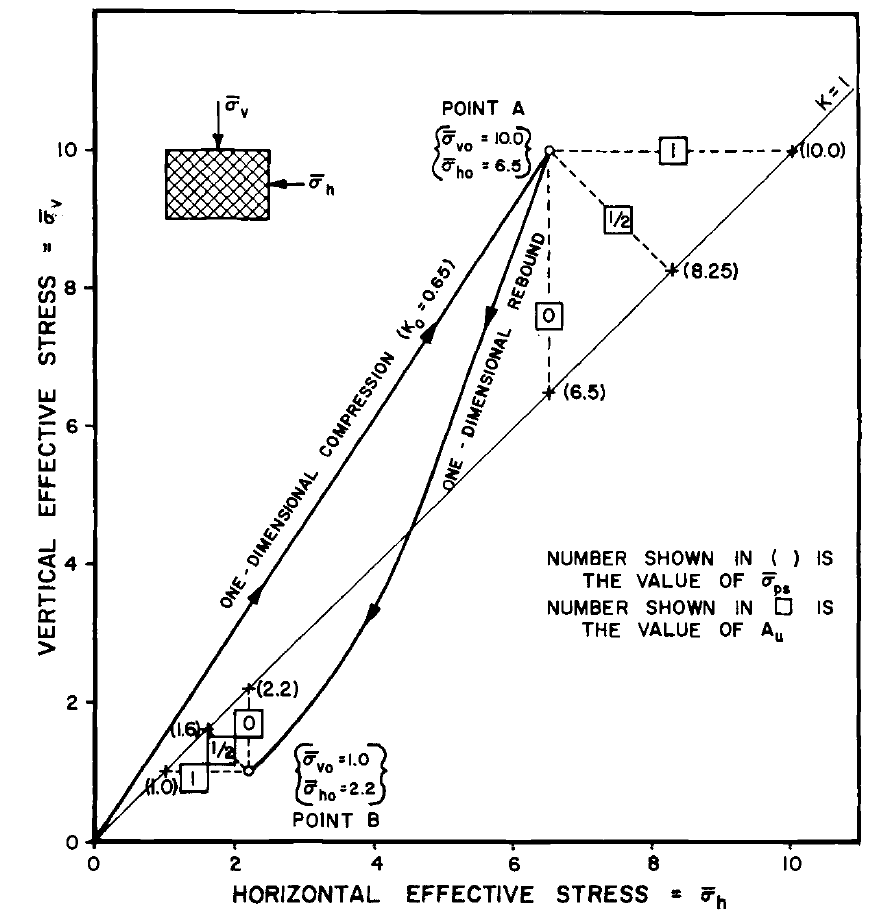
\includegraphics[width=0.5\textwidth]{figures/figure-1.png}\\
    The one-dimensional compression and rebound curves simulate $K_0$ data for the London clay \citet{Skempton1961351}. \\
    一维压缩和回弹曲线模拟了伦敦黏土citet{Skempton1961351}的$K_0$数据。
    \caption{Perfect Sampling of a Normally Consolidated Clay and an Over-consolidated Clay.}
    \addtocounter{figure}{-1}
    \vspace{-5pt}
    \renewcommand{\figurename}{图}
    \caption{正常固结土和超固结土的完美采样。}
    \renewcommand{\figurename}{Figure}
    \label{figure:1}
\end{figure}

\begin{paracol}{2}
    
    \autoref{figure:2} illustrates the effects of perfect sampling on stress paths for a group of clays from Kawasaki, Japan. Pairs of specimens were normally consolidated second specimen was first unloaded by decreasing the axial pressure (that is, perfect sampling), and then loaded by increasing the axial pressure with both steps being done under undrained conditions with pore pressure measurements ($CA-\overline{UU}$ test). The resulting values of the ratio $\overline{\sigma}_{ps}/\overline{\sigma}_{1c}$ were $0.56\pm{}0.05$ with corresponding $A_u$ values of $0.17\pm{}0.10$. Similar test data on normally consolidated Boston Blue Clay (plasticity index = 14 percent; $K_0\approx{}0.54$) yielded $\overline{\sigma}_{ps}/\overline{\sigma}_{1c}=0.59$ and $A_u= 0.11$.

    \switchcolumn

    \cnfigureref{figure:2}说明了完美采样对一组来自日本Kawasaki的黏土的应力路径的影响。 成对的样品通常是固结的,第二个样品首先通过降低轴向压力来卸载(即完美采样),然后通过在不排水条件下利用孔隙压力测量($CA-\overline{UU}$试验)完成两个步骤来增加轴向压力来进行加载 。$\overline{\sigma}_{ps}/\overline{\sigma}_{1c}$之比的所得值为$0.56\pm{}0.05$,相应的$A_u$值为$0.17\pm{}0.10$。 在正常固结的波士顿蓝黏土上的类似试验数据(塑性指数=$14\%$; $K_0\approx{}0.54$)得出$\overline{\sigma}_{ps}/\overline{\sigma}_{1c}=0.59$和$A_u= 0.11$。

\end{paracol}

\begin{figure}[!htb]
    \centering
    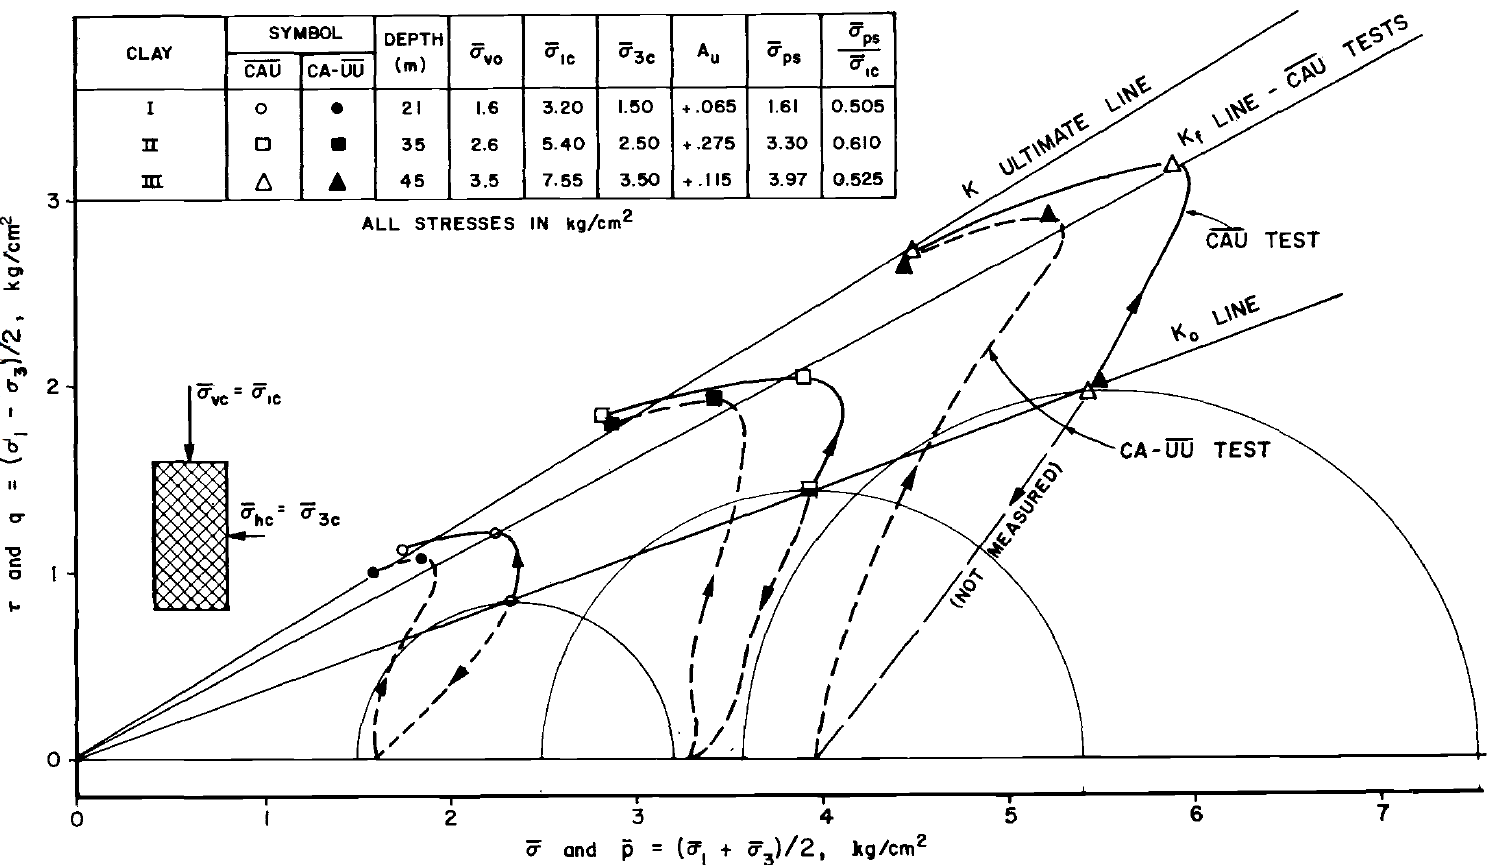
\includegraphics[width=0.8\textwidth]{figures/figure-2.png}
    \caption{Effect of Perfect Sampling on Stress Paths for Normally Consolidated Kawasaki Clays.}
    \addtocounter{figure}{-1}
    \vspace{-5pt}
    \renewcommand{\figurename}{图}
    \caption{完美采样对正常固结的川崎黏土应力路径的影响。}
    \renewcommand{\figurename}{Figure}
    \label{figure:2}
\end{figure}

\begin{paracol}{2}
    
    What are thought to be typical values of $K_0$, $A_u$, and $\overline{\sigma}_{ps}/\overline{\sigma}_{v0}$ are suggested in \autoref{table:1} based on the above and other rather limited data by \citet{Bishop195394} and \citet{Skempton1961351}. As shown in \autoref{table:1}, the effective stress of perfect samples will be only 35 to 80 percent of the in-situ vertical effective stress $\overline{\sigma}_{v0}$ for normally consolidated clays, but may be double $\overline{\sigma}_{v0}$ for a highly overconsolidated plastic clay.

    \switchcolumn

    在\cntableref{table:1}中,根据\citet{Bishop195394}和\citet{Skempton1961351}的上述以及其他相当有限的数据,在\cntableref{table:1}中提出了被认为是$K_0$,$A_u$和$\overline{\sigma}_{ps}/\overline{\sigma}_{v0}$的典型值。 如表一所示,对于正常固结的黏土,理想样品的有效应力仅为原位垂直有效应力的35$\%$至80$\%$,而对于高度超固结的塑料黏土,其有效应力可能是$\overline{\sigma}_{v0}$的两倍。

\end{paracol}

\begin{table*}[!htb]
    \centering
    \caption{STRESS RATIOS FOR PERFECT SAMPLING.}
    \addtocounter{table}{-1}
    \vspace{-8pt}
    \renewcommand{\tablename}{表}
    \caption{完美采样的应力比。}
    \vspace{4pt}
    \renewcommand{\tablename}{Table}
    \begin{tabularx}{\textwidth}{XXXX}
        \toprule
        Type of Specimen & $K_0$ & $A_u$ & $\overline{\sigma}_{ps}/\overline{\sigma}_{v0}$ \\
        \midrule
        Normally consolidated & & & \\
        ~~Clayey Silt & 0.4 to 0.5 & -0.1 to 1 & 0.35 to 0.5 \\
        ~~Lean Clay & 0.5 to 0.6 & ~0.1 to 0.2 & 0.55 to 0.7 \\
        ~~Plastic Clay & 0.6 to 0.7 & ~0.2 to 0.3 & 0.65 to 0.8 \\
        Heavily overconsolidated & & & \\
        ~~Plastic Clay & $\sim$2.5 & $\sim$0.3 & $\sim$2 \\
        \bottomrule
    \end{tabularx}%
    \label{table:1}%
\end{table*}


\Paragraph{Actual Sampling 实际采样}

\begin{paracol}{2}
    
    The ideal sampling process would involve neither a change in moisture content nor a change in magnitude and distribution of effective stresses upon removing a specimen of clay from the field and placing it in the shear test equipment. Such sampling is essentially impossible and the best that can be hoped for is what has been termed in this paper perfect sampling, that is, the removal of the shear stresses acting on the element in tile field to achieve the isotropic stress $\overline{\sigma}_{ps}$. The effects of perfect sampling on the undrained shear behavior in triaxial compression of a normally consolidated clay were illustrated in \autoref{figure:2}.

    \switchcolumn

    理想的采样过程既不涉及水分含量的变化,也不涉及在从现场中取出黏土样本并将其放置在剪切试验设备中时有效应力的大小和分布的变化。 这样的采样基本上是不可能的,可以期望的最好是本文中所称的完美采样,即消除作用在瓷砖场中元素上的剪应力,以实现各向同性应力$\overline{\sigma}_{ps}$。 理想采样对正常固结黏土三轴压缩中不排水剪切行为的影响如\cnfigureref{figure:2}所示。

    \switchcolumn*

    The actual sampling process offers many opportunities for additional disturbance of the soil structure according to \citet{Rutledge19441155}, \citet{Hansen1948189} and \citet{Hvorslev1949}. Some of these effects are illustrated in \autoref{figure:3}, which presents a hypothetical stress path for an element of normally consolidated clay during tube sampling. The Point P with an effective stress of $\overline{\sigma}_{ps}$, corresponds to perfect sampling, whereas Point G with an effective stress of $\overline{\sigma}_r$ represents the effective stress of an actual specimen at the start of a UU shear test. It is proposed that the ratio $\overline{\sigma}_r/\overline{\sigma}_{ps}$ is a measure of the amount of additional disturbance caused by actual sampling.

    \switchcolumn
   
    根据\citet{Rutledge19441155},\citet{Hansen1948189}和\citet{Hvorslev1949}的说法,实际的采样过程为土壤结构的其他扰动提供了许多机会。 其中一些效果如\cnfigureref{figure:3}所示,它为试管采样过程中正常固结的黏土元素提供了假设的应力路径。 有效应力为$\overline{\sigma}_{ps}$的点P对应于完美采样,而有效应力为$\overline{\sigma}_r$的点G表示在UU剪切试验开始时实际样品的有效应力。 建议比率$\overline{\sigma}_r/\overline{\sigma}_{ps}$是对实际采样引起的附加干扰量的度量。

\end{paracol}

\begin{figure}[!htb]
    \centering
    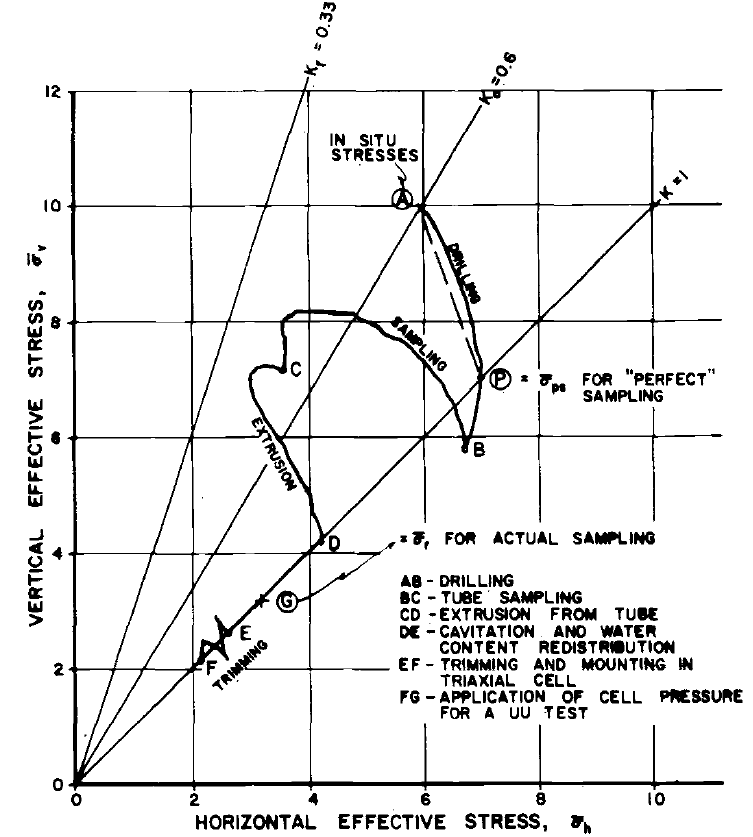
\includegraphics[width=0.5\textwidth]{figures/figure-3.png}
    \caption{Hypothetical Stress Path for a Normally Consolidated Clay Element During Tube Sampling.}
    \addtocounter{figure}{-1}
    \vspace{-5pt}
    \renewcommand{\figurename}{图}
    \caption{管道采样期间正常固结黏土单元的假设应力路径。}
    \renewcommand{\figurename}{Figure}
    \label{figure:3}
\end{figure}

\begin{paracol}{2}
    
    Measured values of the residual effec tive stress after sampling, $\overline{\sigma}_r$, are presented in \cnfigureref{figure:4} for an overconsolidated deposit of Boston Blue Clay and for normally consolidated strata of Kawasaki clays (see \cntableref{table:2} for further data on these clay deposits). The apparatus for UU tests described in the next section was used to measure $\overline{\sigma}_r$ with a total chamber pressure generally between 1 and 3 $\rm{kg/cm^2}$, for which the B parameter became essentially equal to unity. Values of the maximum past pressure, $\overline{\sigma}_{vm}$, in-situ vertical effective stress, $\overline{\sigma}_{v0}$, and effective stress for perfect sampling, $\overline{\sigma}_{ps}$,, are shown for comparison. The ratio $\overline{\sigma}_r/\overline{\sigma}_{ps}$, which is proposed as a measure of the degree of excessive disturbance, ranged from 0.11 to 0.43 with an average value of 0.28 for the Kawasaki clays. Values of $\overline{\sigma}_r/\overline{\sigma}_{ps}$ for the deposit of Boston Blue Clay, which ranged from 0.01 to 0.34, showed a marked decrease with increasing depth and decreasing overconsolidation ratio. Partial drying of the deepest specimen of Boston Blue Clay (depth = 26.2m) revealed a grossly distorted structure which corroborates the very low value of $\overline{\sigma}_r$ of only 0.02 $\rm{kg/cm^2}$. Data from two UU tests on normally consolidated Lagunillas clay (case B in \autoref{table:2}) yielded values of $\overline{\sigma}_r/\overline{\sigma}_{ps}$, equal to $0.36\pm{}0.07$.

    \switchcolumn

    \cnfigureref{figure:4}给出了波士顿蓝黏土超固结沉积物和Kawasaki黏土正常固结地层的采样后残余有效应力的测量值$\overline{\sigma}_r$(有关这些黏土沉积物的更多数据,请参见\cntableref{table:2})。 下一节中描述的用于UU测试的设备用于测量总腔室压力$\overline{\sigma}_r$,通常在1-3$\rm{kg/cm^2}$之间,对于该腔室,B参数基本上等于1。为了比较,显示了最大过去压力$\overline{\sigma}_{vm}$,原位垂直有效应力$\overline{\sigma}_{v0}$和完美采样的有效应力$\overline{\sigma}_{ps}$的值。作为对过度扰动程度的一种度量,提出的比率$\overline{\sigma}_r/\overline{\sigma}_{ps}$在0.11至0.43的范围内,Kawasaki黏土的平均值为0.28。 波士顿蓝土沉积物的$\overline{\sigma}_r/\overline{\sigma}_{ps}$值在0.01到0.34之间,随深度增加和过固结率降低而显着降低。波士顿蓝黏土的最深标本(深度为26.2m)的部分干燥显示出严重扭曲的结构,这证实了其仅0.02$\rm{kg/cm^2}$的非常低的$\overline{\sigma}_r$值。 在正常固结的Lagunillas黏土上进行的两次UU测试数据(\cntableref{table:2}中的情况B)得出的$\overline{\sigma}_r/\overline{\sigma}_{ps}$值等于$0.36\pm{}0.07$。

\end{paracol}

\begin{figure}[!htb]
    \centering
    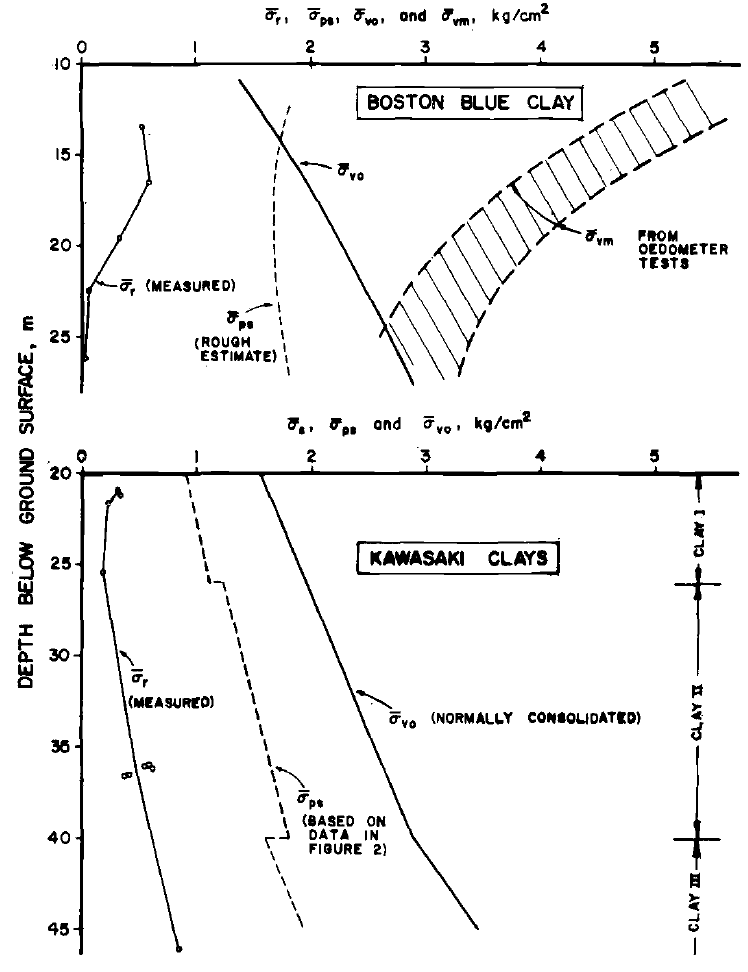
\includegraphics[width=0.5\textwidth]{figures/figure-4.png}
    \caption{Effect of Tube Sampling on Effective Stresses for Boston Blue Clay and the Kawasaki clays.}
    \addtocounter{figure}{-1}
    \vspace{-5pt}
    \renewcommand{\figurename}{图}
    \caption{采样对波士顿蓝黏土和川崎黏土有效应力的影响。}
    \renewcommand{\figurename}{Figure}
    \label{figure:4}
\end{figure}

\begin{table}[!htb]
    \centering
    \scriptsize
    \renewcommand{\arraystretch}{1.2}
    \caption{COMPARISON OF UNDRAINED STRENGTH FROM UU AND CU TESTS.}
    \addtocounter{table}{-1}
    \vspace{-8pt}
    \renewcommand{\tablename}{表}
    \caption{UU和CU试验的不排水强度的比较。}
    \vspace{4pt}
    \renewcommand{\tablename}{Table}
    \begin{threeparttable}[b]
        \setlength{\tabcolsep}{0.4mm}{
        \begin{tabularx}{\textwidth}{lllllllll}
            \toprule
             & & & & \multicolumn{2}{l}{From U or UU Tests} & & & \\
            Case & Location & Description of Clay & Depth, m & $S_u, \rm{kg/cm^2}$ & $S_u/\overline{\sigma}_{v0}$ & $\dfrac{S_u(UU)}{S_u(CIU,\overline{\sigma}_c=\overline{\sigma}_{v0})}$ & Remarks & Source \\
            \midrule
            A & \makecell[tl]{M.I.T., \\~~Cambridge,\\~~Mass}             & \makecell[tl]{o.c.\tnote{a} a Boston blue clay\\o.c. Boston blue clay \\~~~~~~(slightly)\\n.c.\tnote{b} Boston blue clay} & \makecell[tl]{12.2\\18.3\\\\27.4} & \makecell[tl]{0.80\\0.68\\\\0.50} & \makecell[tl]{0.59\\0.37\\\\0.185} & \makecell[tl]{~~0.74\\~~0.77\\\\~~0.58} & \makecell[tl]{3 in. diameter shelby \\~~fixed piston samples} & M.I.T.\\
            B & \makecell[tl]{Lagunillas, \\~~Venezuela}               & \makecell[tl]{n.c. plastic clay \\~~$w_L\cong{}61\%$ \\~~$P.I.\cong{}37\%$} & 6.2 & 0.18 & 0.30 & ~~0.75 & \makecell[tl]{3 in. diameter shelby samples.\\~~$S_u$(UU) based on average \\~~of U and UU data} & M.I.T. \\
            C & \makecell[tl]{Kawasaki, \\~~Japan}                     & \makecell[tl]{normally consolidated \\~~plastic clay \\~~Clay I, P.I.\tnote{c}$\cong{}31\%$\\~~Clay I, P.I. $\cong{}36\%$\\~~Clay II, P.I.$\cong{}43\%$} & \makecell[tl]{\\\\20.5\\25\\35} & \makecell[tl]{\\\\0.50\\0.49\\0.69} & \makecell[tl]{\\\\0.31\\0.26\\0.27} & \makecell[tl]{\\\\~~0.64\\~~0.58\\~~0.57} & \makecell[tl]{3 in. diameter shelby samples.\\~~$S_u$(UU) from top one-third \\~~of U and from UU data \\~~corrected to $t_f=5$ hr} & M.I.T. \\
            D & \makecell[tl]{Gulf of \\Mexico}                          & \makecell[tl]{o.c. soft plastic clay\\~~P.I.$\cong{}80\%$\\~~L.I.$\cong{}50\%$\\firm plastic clay with silt \\~~and sand\\~~P.L.$\cong{}60\%$\\~~L.I.$\cong{}35\%$} & \makecell[tl]{0 to 6 \\\\\\18 to 50} & \makecell[tl]{avg.$\cong{}$0.27\\\\\\acg.$\cong{}$0.50} & \makecell[tl]{...\\\\\\...} & \makecell[tl]{$\sim{}$0.85\\\\\\$\sim{}$0.5} & Shelby samples & \citet{Fenske195616} \\
            E & \makecell[tl]{Skabo, Oslo,\\~~Norway}                  & \makecell[tl]{n.c. plastic clay with a \\~~high salt content\\~~P.I. $\cong{}30\%$\\~~L.I.$\cong{}65\%$\\~~$S_t\cong{}30\%$} & 10.6 to 16 & avg.=0.32 & 0.31 & ~~0.74 & \makecell[tl]{2.1 in. diameter thin walled\\~~fixed piston samples} & \makecell[tl]{N.G.I. Internal\\~~Report No.\\~~F175 (1962)}\\
            F & \makecell[tl]{$\rm{G\ddot{o}ta}$ Valley, \\~~Sweden}   & \makecell[tl]{Lilla Edet Clay\\~~highly  o.c. P.I. $\cong{}30\%$\\~~slightly o.c. P.I.$\cong{}33\%$\\~~slightly o.c. P.I.$\cong{}29\%$\\~~slightly o.c. P.I.$\cong{}37\%$} & \makecell[tl]{\\~~~4 to 6.8\\~~10 to 12.3\\16.2 to 18\\10.8 to 12.8} & \makecell[tl]{\\avg.$\cong{}$0.4\\avg.=0.34\\avg.=0.46\\avg.=0.13} & \makecell[tl]{\\$\sim$1.20\\~~0.45\\~~0.42\\~~0.13} & \makecell[tl]{\\$\sim$0.90\\~~0.60\\~~0.66\\~~0.40} & \makecell[tl]{2.1 in. diameterr thin walled \\~~fixed piston samples. Clay \\~~believed to have a significant \\~~amount of natural \\~~cementation} & \begin{minipage}[t]{1.6cm}\citet{Bjerrum1960101}\end{minipage} \\
            G & \makecell[tl]{Mexico City}                             & \makecell[tl]{Mexico City CLay, \\~~slightly o.c.} & ... & ... & ... & ~~0.74 & ... & \citet{Marsal1957229}\\
            H & \makecell[tl]{Drammen, \\~~Norway}                     & \makecell[tl]{normally consolidated soft \\~~silty clay with thin seams \\~~of silt and fine sand\\~~P.I.$\cong{}8\% S_t=10$\\~~P.I.$\cong{}16\% S_t=9$\\~~P.I.$\cong{}14\% S_t=9$} & \makecell[tl]{\\\\\\~5\\12\\18} & \makecell[tl]{\\\\\\0.25\\0.25\\0.24} & \makecell[tl]{\\\\\\0.37\\0.19\\0.24} & \makecell[tl]{\\\\\\~~0.97\\~~0.57\\~~0.40} & \makecell[tl]{2.1 in. diameter thin walled, \\~~fixed piston samples. $S_u$\\~~(UU) based on U samples \\~~with lowest strain at failure} & \citet{Simons1960727}\\
            I & \makecell[tl]{Sault Ste.\\~~Marir, Mich}               & \makecell[tl]{n.c. varved clay\\~~P.I.$\cong{}28\%$\\~~$S_t\cong{}8$} & $\sim$9 & $\sim$0.3 & $\sim$0.15 & $\sim$0.60 & \makecell[tl]{3.5 in. diameter thin walled \\~~piston. $S_u$(CIU) based on \\~~$S_u/\overline{\sigma}_c$ for $\overline{\sigma}_c>\overline{\sigma}_{v0}$} & \begin{minipage}[t]{1.4cm}\citet{Wu19581, Wu19621}\end{minipage}\\
            \bottomrule
        \end{tabularx}}%
        \begin{tablenotes}
            \item[a] O.C. = overconsolidated.
            \item[b] N.C. = normally consolidated.
            \item[c] P.I. = plasticity index.
        \end{tablenotes}
    \end{threeparttable}  
    \label{table:2}%   
    \renewcommand{\arraystretch}{1.0}
\end{table}


\begin{paracol}{2}
    
    These limited data show that the effective stress of laboratory specimens of normally consolidated and slightly overconsolidated clays after tube sampling may be lowered by excessive disturbance to a value of only $20\pm20$ percent of the theoretical value for perfect sampling. It is therefore suggested that the measurement of the residual effective stress, $\overline{\sigma}_r$, of laboratory specimens should become a standard test for jobs requiring a rational interpretation of lab strength data, especially for deep tube samples of normally consolidated clay. The value of $\overline{\sigma}_r$ can be obtained from a direct measurement of the residual pore pressure $u_r$, (that is, $u$ at zero confining pressure; \cite{Lambe1961207} describes several methods for measuring $u_r$) provided that $\overline{\sigma}_r$ is less than one atmosphere, although the use of a confining pressure of several atmospheres is preferable since the B parameter is generally some-what less than unity.\footnote{
        In this case UU tests with a confining pressure sufficient to make B equal unity are preferable to unconfined compression tests. 在这种情况下,UU试验的围压足以使B等于1,优于无限制压缩试验。
    } \citet{Skempton1961351} suggests some indirect methods for evaluating $\overline{\sigma}_r$.

    \switchcolumn

    这些有限的数据表明,由于过度扰动,正常固结和稍固结的粘土的实验室标本的有效应力可能会由于过度干扰而降低,仅为理想采样的理论值的$20\%\pm{}20\%$。 因此,建议对于需要合理解释实验室强度数据的工作,特别是对于通常固结的粘土的深管样品,对实验室样品的残余有效应力$\overline{\sigma}_r$的测量应成为标准测试。$\overline{\sigma}_r$的值可以通过直接测量残余孔隙压力$u_r$(即$u$在零围压下; \cite{Lambe1961207}描述了几种测量$u_r$的方法)获得,前提是$\overline{\sigma}_r$小于一个大气压,尽管最好使用几个大气压的限制压力,因为B参数通常略小于1。\citet{Skempton1961351}提出了一些间接的方法来评估$\overline{\sigma}_r$。

    \switchcolumn*

    Experience at Massachusetts Institute of Technology has shown, for example, that the size of the specimen, the amount of trimming, and the placement of the specimen in an oedometer ring can affect the value of $\overline{\sigma}_r$. In other words, the value of $\overline{\sigma}_r$, and hence the degree of disturbance, are really variables.

    \switchcolumn

    麻省理工学院的经验表明,例如,标本的大小,修整量以及标本在里程表环中的放置都会影响$\overline{\sigma}_r$的值。 换句话说,$\overline{\sigma}_r$的值以及扰动程度实际上是变量。

\end{paracol}
\section{COMPARISON OF UU AND CU TEST RESULTS UU和CU试验结果的比较}

\begin{paracol}{2}
    
    \autoref{table:2} presents test data on nine soils from various locations in the world. Most of the soils are normally consolidated or slightly overconsolidated, $\overline{\sigma}_{vm}/\overline{\sigma}_{v0}$ equal to less than 3, lean to plastic clays with sensitivities below ten. Specimen depths varied from 0 to 35 m below ground surface. The strength values in Columns 4 and 5 are the averages from unconfined (U tests) and UU triaxial compression tests except for Case C as noted. The results of vane tests were not included in \autoref{table:2} since the interpretation of vane data is open to question.\footnote{
        The ratio of $S_u$ (UU) to vane strength averaged 0.85 (0.45 to 2.0) for Cases B, C, D, F, H, and I in \autoref{table:2}. \cntableref{table:2}中的情况B,C,D,F,H和I的$S_u$(UU)与叶片强度的比率平均为0.85(0.45至2.0)。
    }

    \switchcolumn

    \cntableref{table:2}列出了来自世界各地的9种土体的试验数据。 大多数土体通常是固结的或略有过固结的,$\overline{\sigma}_{vm}/\overline{\sigma}_{v0}$等于3以下,通常为敏感度低于10的塑料黏土。 标本深度在地面以下0到35 m之间变化。 第4列和第5列中的强度值是无限制(U试验)和UU三轴压缩试验的平均值,但情况C除外。 叶片试验的结果未包含在\cntableref{table:2}中,因为叶片的数据值得商榷。

    \switchcolumn*

    As Column 6 of \autoref{table:2} shows, the undrained strength as obtained from UU tests varies from 40 to 97 percent of the strength as obtained from CIU tests with $\overline{\sigma}_c=\overline{\sigma}_{v0}$, with an average value of 66 percent. In general, this ratio decreased with increasing depth of specimen.

    \switchcolumn

    如\cntableref{table:2}的第6列所示,UU试验获得的不排水强度$\overline{\sigma}_c=\overline{\sigma}_{v0}$时CIU试验获得的不排水强度的40$\%$至97$\%$,平均值为66$\%$。 通常,该比率随样品深度的增加而降低。

    \switchcolumn*

    A more detailed comparison of the results of $\overline{UU}$ and $\overline{CIU}$ tests on the Lagunillas clay, Case B of \autoref{table:2}, and the Kawasaki clays, Case C of \autoref{table:2}, is given in \autoref{figure:5} to \autoref{figure:10}. The tests on these normally consolidated clays were run on trimmed specimens 10 $\rm{cm^2}$ in area by 8 cm high using either the Norwegian Geotechnical Inst. (NGI) equipment \citep{Andresen1960695} or English equipment \citep{Bishop1962}. The NGI null device was used for the $\overline{CIU}$ tests; filter strips were placed on the test specimens, and backpressures of 1 to 3 $\rm{kg/cm^2}$ were employed. The rate of strain was about 1 percent/hr. A filter strip correction of 0.10 $\rm{kg/cm^2}$ was subtracted from measured values of ($\sigma_1-\sigma_3$) for axial strains exceeding 2 percent. The UU tests employed a fine porous base stone and Dynisco pressure transducer \citep{Whitman1961407}, no filter strips, a cell pressure of several $\rm{kg/cm^2}$, and a time to failure generally exceeding one day. All triaxial specimens were encased with two prophylactics with silicone grease; measured values of the B parameter before shear always exceeded 0.95 within 2 min. 

    \switchcolumn

    在\cntableref{table:2}的情况B的Lagunillas黏土和\cntableref{table:2}的情况C的Kawasaki黏土的$\overline{UU}$和$\overline{CIU}$试验结果的更详细比较在\cnfigureref{figure:5}至\cnfigureref{figure:10}。这些正常固结的黏土的试验是使用挪威岩土工程学院在面积10$\rm{cm^2}$高8cm的修整试样上进行的。 使用Norwegian Geotechnical Inst(NGI)设备\citep{Andresen1960695}或English设备\citep{Bishop1962}。NGI空设备用于$\overline{CIU}$试验; 将滤纸条放在试样上,并使用1至3$\rm{kg/cm^2}$的背压。 应变率约为1$\%$/小时。 如果轴向应变超过2$\%$,则从($\sigma_1-\sigma_3$)的测量值中减去0.10$\rm{kg/cm^2}$的滤带校正量。  UU试验使用了细的多孔基石和Dynisco压力传感器\citep{Whitman1961407},没有过滤带,电池压力为几$\rm{kg/cm^2}$,并且失效时间通常超过一天。 所有三轴试样均用硅脂润滑脂包裹了两种预防措施,剪切前B参数的测量值在2分钟内始终超过0.95。

    \begin{figure*}[!htbp]
    \centering
    \begin{minipage}[t]{0.48\textwidth}
        \centering
        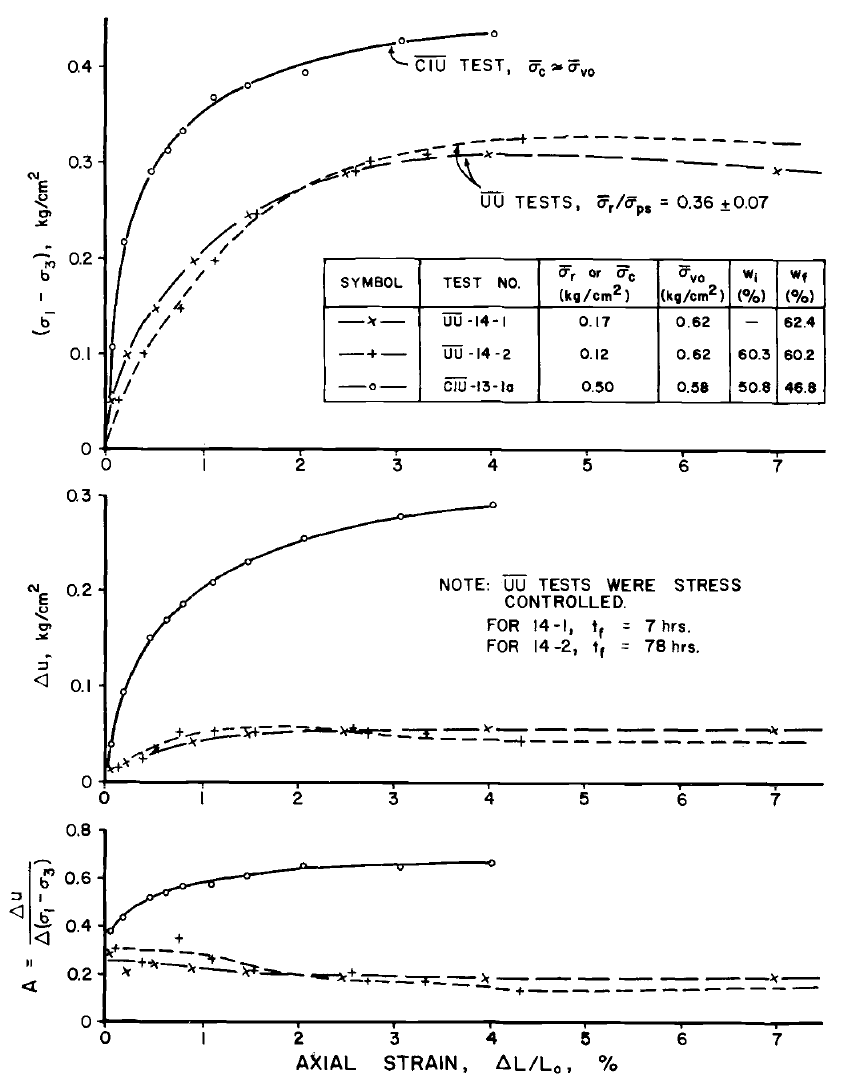
\includegraphics[width=0.9\textwidth]{figures/figure-5.png}
        \caption{Stress-Strain Data from Triaxial Tests on Lagunilas Clay.}
        \vspace{-5pt}
        \addtocounter{figure}{-1}
        \renewcommand{\figurename}{图}
        \caption{Lagunilas黏土的三轴试验的应力应变数据。}
        \label{figure:5}
        \renewcommand{\figurename}{Figure}
    \end{minipage}
    \begin{minipage}[t]{0.48\textwidth}
        \centering
        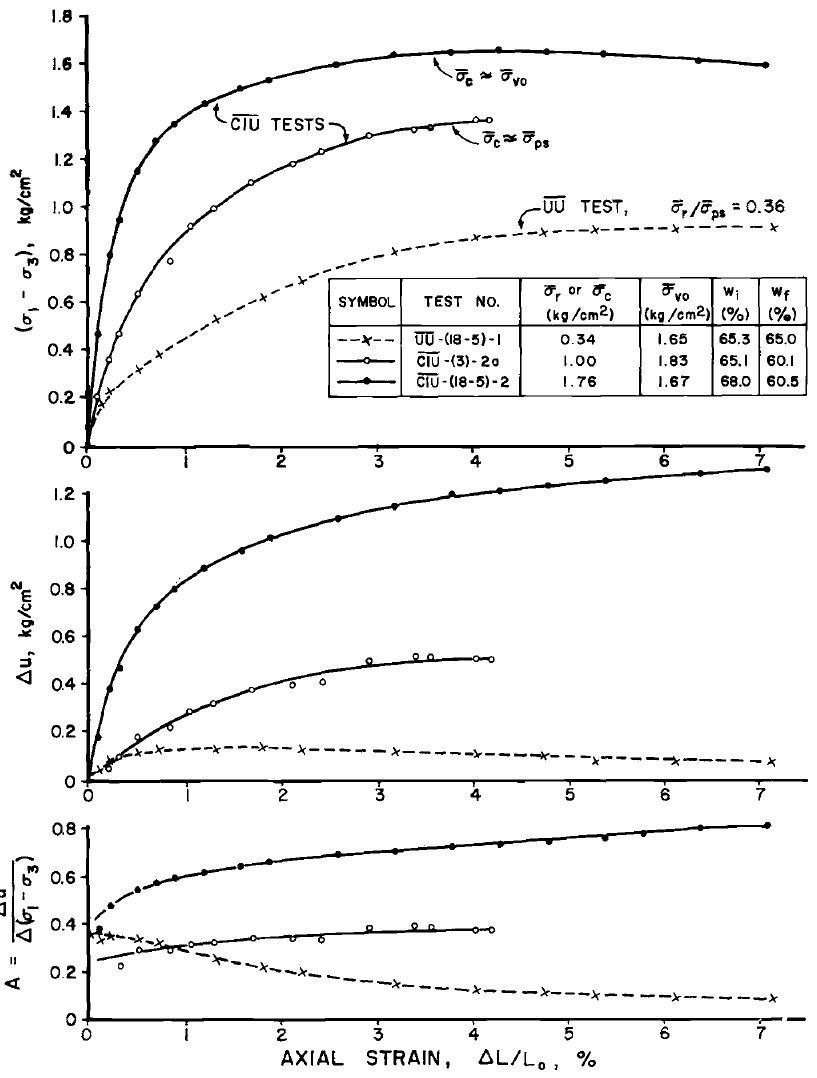
\includegraphics[width=0.9\textwidth]{figures/figure-6.png}
        \caption{Stress-Strain Data from Triaxial Tests on Kawasaki Clay I}
        \vspace{-5pt}
        \addtocounter{figure}{-1}
        \renewcommand{\figurename}{图}
        \caption{川崎黏土I的三轴试验的应力应变数据。}
        \label{figure:6}
        \renewcommand{\figurename}{Figure}
    \end{minipage}
\end{figure*}

    \begin{figure*}[!htbp]
    \centering
    \begin{minipage}[t]{0.48\textwidth}
        \centering
        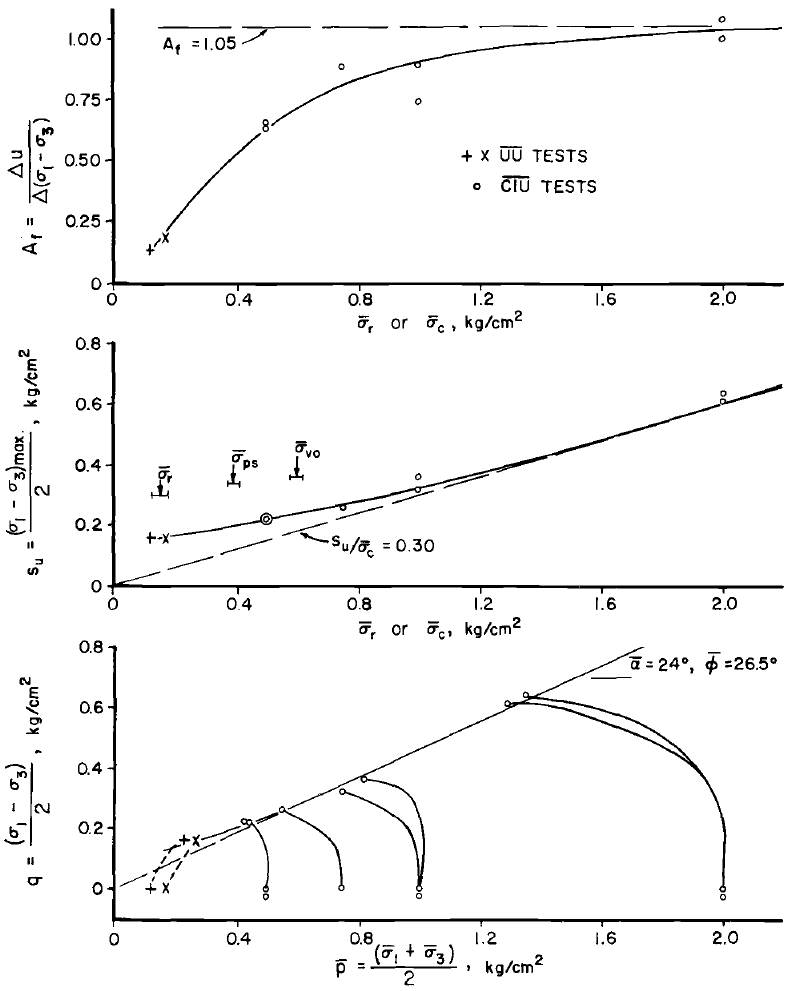
\includegraphics[width=0.9\textwidth]{figures/figure-7.png}
        \caption{Strength Data from Triaxial Tests on Lagunilas Clay.}
        \vspace{-5pt}
        \addtocounter{figure}{-1}
        \renewcommand{\figurename}{图}
        \caption{Lagunilas黏土的三轴试验的强度数据。}
        \label{figure:7}
        \renewcommand{\figurename}{Figure}
    \end{minipage}
    \begin{minipage}[t]{0.48\textwidth}
        \centering
        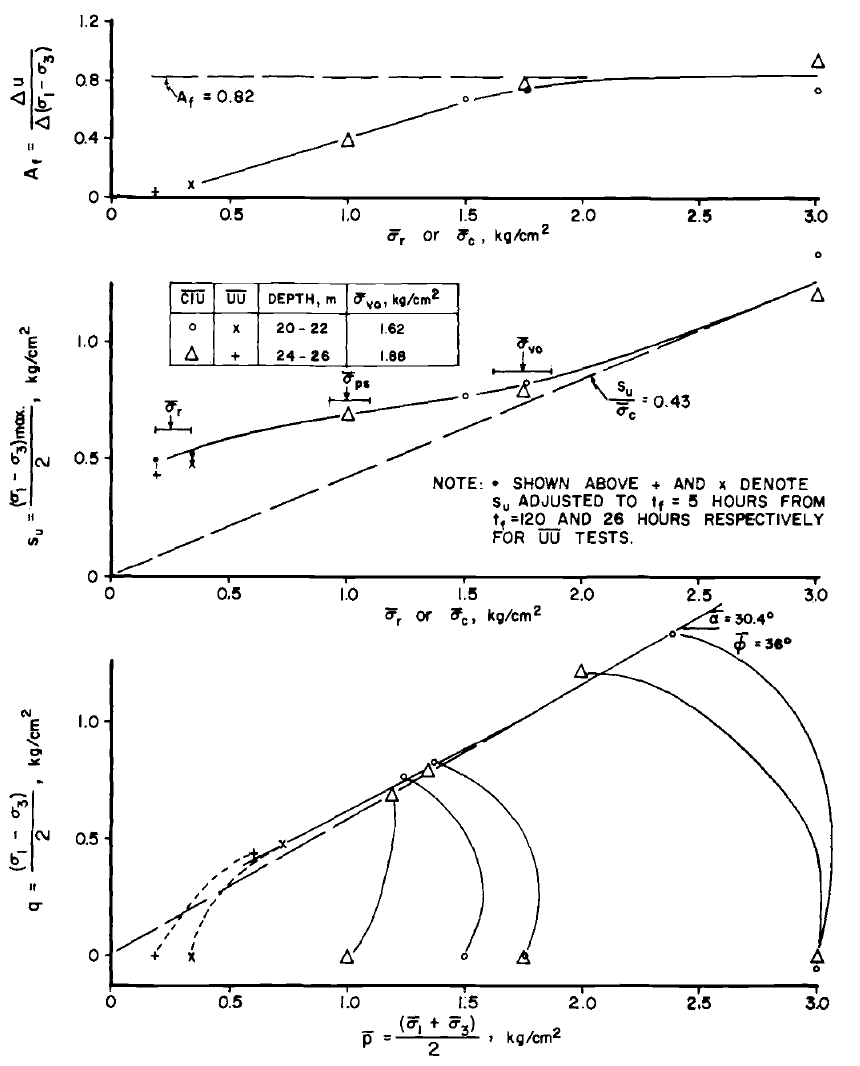
\includegraphics[width=0.9\textwidth]{figures/figure-8.png}
        \caption{Strength Data from Triaxial Tests on Kawasaki Clay I}
        \vspace{-5pt}
        \addtocounter{figure}{-1}
        \renewcommand{\figurename}{图}
        \caption{川崎黏土I的三轴试验的强度数据。}
        \label{figure:8}
        \renewcommand{\figurename}{Figure}
    \end{minipage}
\end{figure*}
    \begin{figure*}[!htbp]
    \centering
    \begin{minipage}[t]{0.48\textwidth}
        \centering
        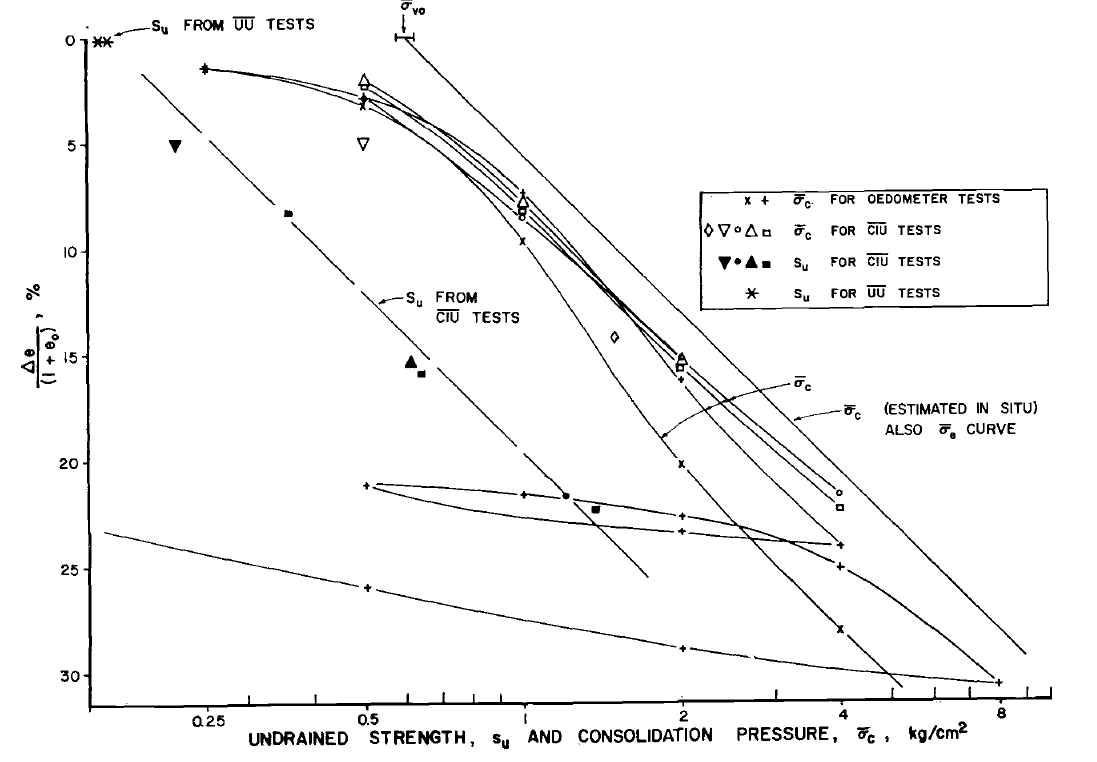
\includegraphics[width=0.9\textwidth]{figures/figure-9.png}
        \caption{Strength and Consolidation Pressure Versus Volumetric Strain on Lagunilas Clay.}
        \vspace{-5pt}
        \addtocounter{figure}{-1}
        \renewcommand{\figurename}{图}
        \caption{Lagunilas的黏土强度和固结压力与体积应变。}
        \label{figure:9}
        \renewcommand{\figurename}{Figure}
    \end{minipage}
    \begin{minipage}[t]{0.48\textwidth}
        \centering
        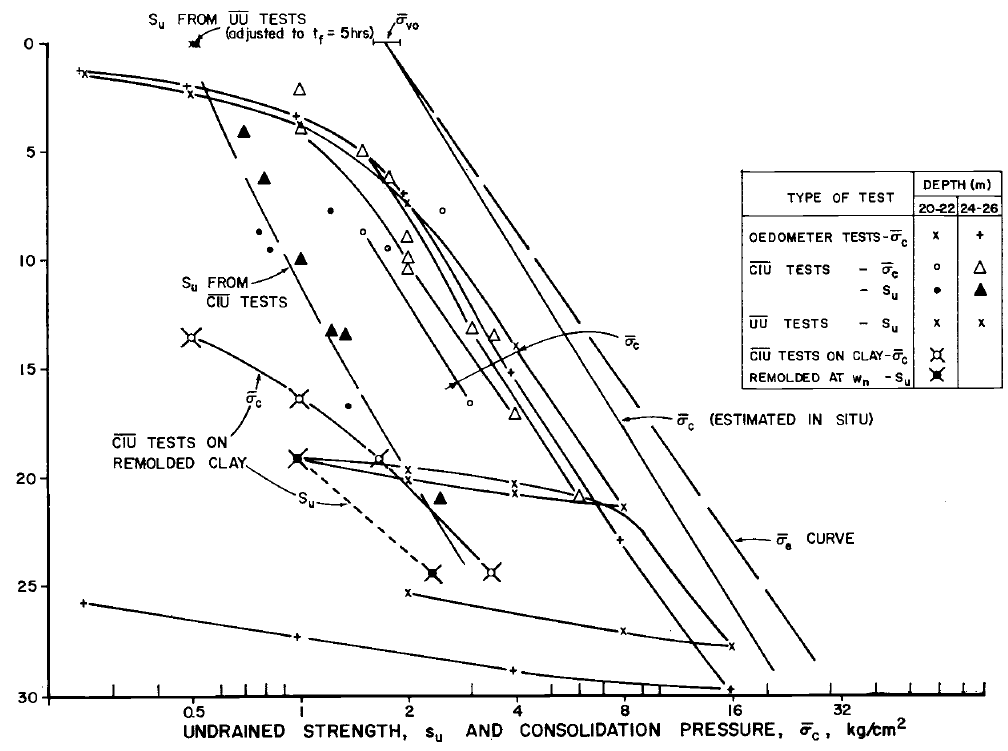
\includegraphics[width=0.9\textwidth]{figures/figure-10.png}
        \caption{Strength and Consolidation Pressure Versus Volumetric Strain on Kawasaki Clay I}
        \vspace{-5pt}
        \addtocounter{figure}{-1}
        \renewcommand{\figurename}{图}
        \caption{Lagunilas黏土I的强度和固结压力与体积应变。}
        \label{figure:10}
        \renewcommand{\figurename}{Figure}
    \end{minipage}
\end{figure*}
    \switchcolumn*

    The data in \autoref{figure:5} through \autoref{figure:10} show the following results:\footnote{
        Measured or estimated values of $\overline{\sigma}_r$, $\overline{\sigma}_{ps}$ and $\overline{\sigma}_{v0}$ are generally shown in the figures for reference. $\overline{\sigma}_r$,$\overline{\sigma}_{ps}$和$\overline{\sigma}_{v0}$的测量或估计值通常在图中显示,以供参考。
    }

    \switchcolumn
    
    从\cnfigureref{figure:5}至\cnfigureref{figure:10}中的数据可得出以下结果:

    \switchcolumn*

    \begin{enumerate}
        \item The undrained shear strength, $S_u$, from $\overline{UU}$ tests is only 70 to 85 percent of the value from $\overline{CIU}$ tests consolidated to the theoretical pressure corresponding to perfect sampling, that is, $\overline{\sigma}_c=\overline{\sigma}_{ps}$, (\autoref{figure:7} and \autoref{figure:8}). This difference in $S_u$ arises from the fact that the residual effective stress $\overline{\sigma}_r$, of the laboratory shear specimens is considerably less than the theoretical value $\overline{\sigma}_{ps}$. Identical strengths would have resulted if $\overline{\sigma}_r$, had equalled $\overline{\sigma}_{ps}$ since the preshear $\overline{\sigma}$ and void ratios would therefore have been equal for both tests.
        \item The slope of the stress-strain curve from $\overline{UU}$ tests is approximately one half of that from $\overline{CIU}$ tests with $\overline{\sigma}_c=\overline{\sigma}_{ps}$ (\autoref{figure:5} and \autoref{figure:6}).
        \item  There is good agreement among $\overline{UU}$ and $\overline{CIU}$ strength data if the $\overline{CIU}$ data are extrapolated backward so that the consolidation pressure equals $\overline{\sigma}_r$ (\autoref{figure:7} and \autoref{figure:8}) or the volumetric strain from the field condition is zero (\autoref{figure:9} and \autoref{figure:10}). This is to be expected since as the $\overline{\sigma}_c$ of $\overline{CIU}$ tests increased beyond $\overline{\sigma}_r$, there are corresponding increases in preshear $\overline{\sigma}$ and volumetric strain.
        \item As the consolidation pressure of $\overline{CIU}$ tests is increased from $\overline{\sigma}_{ps}$ to several times the in-situ vertical effective stress $\overline{\sigma}_{v0}$, $A_f$ shows a large increase and $S_u/\overline{\sigma}_c$ exhibits a marked decrease, whereas changes in the effective stress envelope are relatively minor (\autoref{figure:7}和\autoref{figure:8}).
        \item A relatively large volume decrease occurs when specimens are isotropically consolidated to pressures between $\overline{\sigma}_{ps}$ and $\overline{\sigma}_{v0}$ (\autoref{figure:9} and \autoref{figure:10}). Moreover, the oedometer test data\footnote{
        The fact that one of the oedonmter test eversus log$\overline{\sigma}_c$ curves in \autoref{figure:9} fell considerably below the curves for isotropic consolidation at high pressures is not considered typical. \cnfigureref{figure:9}中的oedonmter检验曲线log$\overline{\sigma}_c$曲线之一大大低于高压下的各向同性固结曲线,这一事实被认为是不典型的。
    } show that low values of $S_u/\overline{\sigma}_r$, indicating high disturbance, rather than an isotropic stress system \textit{per se}, are primarily responsible for the volume decrease.
    \end{enumerate}

    \switchcolumn

    \begin{enumerate}
        \item $\overline{UU}$试验的不排水剪切强度$S_u$仅为$\overline{CIU}$试验的固结至理论压力的70$\%$至85$\%$,即对应于完美采样的理论压力,即$\overline{\sigma}_c=\overline{\sigma}_{ps}$(\cnfigureref{figure:7}和\cnfigureref{figure:8})。$S_u$的差异是由于实验室剪切试样的残余有效应力$\overline{\sigma}_c$远小于理论值$\overline{\sigma}_{ps}$。 如果$\overline{\sigma}_c$等于$\overline{\sigma}_{ps}$,将产生相同的强度,因为预剪切力$\overline{\sigma}$和空隙率因此在两个试验中均相等。
        \item 若$\overline{\sigma}_c=\overline{\sigma}_{ps}$,$\overline{UU}$试验的应力-应变曲线的斜率约为$\overline{CIU}$试验的斜率的一半(\cnfigureref{figure:5}和\cnfigureref{figure:6})。
        \item 如果将$\overline{CIU}$数据向后外推,以使固结压力等于$\overline{\sigma}_r$(\cnfigureref{figure:7}和\cnfigureref{figure:8})或现场条件下的体积应变为零(\cnfigureref{figure:9}和\cnfigureref{figure:10}),则$\overline{UU}$和$\overline{CIU}$强度数据之间存在很好的一致性。这是可以预期的,因为随着$\overline{CIU}$试验的$\overline{\sigma}_c$增加到$\overline{\sigma}_r$以上,预剪力$\overline{\sigma}$和体积应变也会相应增加。
        \item 随着$\overline{CIU}$试验的固结压力从$\overline{\sigma}_{ps}$增加到原位垂直有效应力$\overline{\sigma}_{v0}$的几倍,$A_f$值显示出较大的增加,而$S_u/\overline{\sigma}_c$则显示出明显的降低,而有效应力包络线的变化相对较小(\cnfigureref{figure:7}和\cnfigureref{figure:8})。
        \item 当样品各向同性固结到$\overline{\sigma}_{ps}$和$\overline{\sigma}_{v0}$之间的压力时,体积会相对减小(\cnfigureref{figure:9}和\cnfigureref{figure:10})。此外,里程表试验数据表明,低值$S_u/\overline{\sigma}_r$表示高干扰,而不是各向同性应力系统本身,是体积减小的主要原因。
    \end{enumerate}

    \switchcolumn*
    
    These five trends are believed to be typical of tube specimens of normally consolidated, moderately sensitive, plastic clays which do not possess significant natural cementation.

    \switchcolumn
    
    这五个趋势被认为是通常固结,中等敏感性,不具有明显天然胶结作用的塑料黏土的试管样品的典型特征。

    \switchcolumn*

    \emph{In summary:} 

    \switchcolumn

    \emph{综上所述:}

    \switchcolumn*

    \begin{enumerate}
        \item Disturbance during tube sampling of normally consolidated clays may commonly decrease the effective stress of lab specimens by $80\pm{}20$ percent compared to perfect sampling.
        \item The resultant low values of $\overline{\sigma}_r$ cause the undrained strength $S_u$ from UU tests to be too low, whereas $S_u$ from CIU tests, which experience a significant volume decrease during consolidation, will most likely be too large.
        \item The ratio of $S_u$ from UU tests to that from CIU tests with $\overline{\sigma}_c=\overline{\sigma}_{ps}$ will typically be $75\pm{}25$ percent.
    \end{enumerate}

    \switchcolumn

    \begin{enumerate}
        \item 与完全采样相比,正常固结黏土的采样期间的干扰通常可能会使实验室标本的有效应力降低$80\%\pm{}20\%$。
        \item 所得的$\overline{\sigma}_r$值较低,导致UU试验的不排水强度$S_u$太低,而CIU试验的$S_u$则在固结过程中体积明显减小,很可能太大。
        \item $\overline{\sigma}_c=\overline{\sigma}_{ps}$的UU试验与CIU试验的$S_u$比率通常为$75\%\pm{}25\%$。
    \end{enumerate}

\end{paracol}
\section{EXAMINATION OF THE UNCONSOLIDATED-UNDRAINED TEST 不固结不排水试验试验\protect\footnote[6]{
    The following two sections on UU and CU Tests are restricted to normally consolidated clays of moderate sensitivity, although the concepts can be extended to overconsolidated clays. 以下有关UU和CU试验的两节仅限于中等敏感度的正常固结黏土,尽管这些概念可以扩展到超固结黏土。
}}

\begin{paracol}{2}
    
    The test data in \autoref{figure:5} through \autoref{figure:8} indicate that soil tested in unconsolidatedundrained shear resembles, in several respects, the results of tests on overconsolidated clays. In particular, the $\overline{UU}$ data show: 

    \switchcolumn

    图中的试验数据。 \cnfigureref{figure:5}至\cnfigureref{figure:8}表明,在非固结不排水的剪切中试验的土壤在某些方面类似于对超固结黏土的试验结果。 特别是,$\overline{UU}$数据显示:

    \switchcolumn*

    \begin{enumerate}
        \item Values of undrained shear strength for a given initial effective stress $\overline{\sigma}_r$ which are above the corresponding values for normally consolidated clay; 
        \item Effective stress paths during shear which move upward and to the right since the pore pressure parameter $A$ is less than one half, a characteristic of overconsolidated clay;
    \end{enumerate}

    \switchcolumn
    
    \begin{enumerate}
        \item 对于给定的初始有效应力$\overline{\sigma}_r$,不排水的剪切强度值高于正常固结黏土的相应值; 
        \item 由于孔隙压力参数$A$小于1/2,因此在剪切过程中有效应力路径向上和向右移动,这是黏土的超固结特征。 
    \end{enumerate}

    \switchcolumn*
    
    The similarity between the results of $\overline{UU}$ tests and tests on overconsolidated specimens is presented in \autoref{figure:11} for Kawasaki clays. In \autoref{figure:11b} $CA-\overline{UU}$ tests represent the undrained strength of perfect specimens, preshear $\overline{\sigma}=\overline{\sigma}_{ps}$, whereas the UU tests show the strength of actual specimens, preshear $\overline{\sigma}=\overline{\sigma}_r$. This figure shows that the effective stress paths for the $\overline{UU}$ tests, \autoref{figure:11b}, when normalized by dividing by $\overline{\sigma}_{ps}$, are similar in shape to the effective stress paths of 的$\overline{CIU}$ tests on overconsolidated clays shown in \autoref{figure:11a}, when normalized by dividing by $\overline{\sigma}_{cm}$. In other words, the reduction in effective stress from $\overline{\sigma}_{ps}$ to $\overline{\sigma}_r$ caused by sample disturbance and the reduction in effective stress from $\overline{\sigma}_{cm}$ to $\overline{\sigma}_c$ caused by rebound appear to have comparable effects on undrained strength.

    \switchcolumn
    
    对于Kawasaki黏土,$\overline{UU}$试验结果与超固结试样试验之间的相似性在\cnfigureref{figure:11}中给出。 在\cnsubfigureref{figure:11b}中,$CA-\overline{UU}$试验代表理想试样的不排水强度,预剪切力$\overline{\sigma}=\overline{\sigma}_{ps}$,而$\overline{UU}$试验则表明实际试样的强度,预剪切力$\overline{\sigma}=\overline{\sigma}_r$。 该图表明,通过除以$\overline{\sigma}_{ps}$进行归一化后,$\overline{UU}$试验的有效应力路径\cnsubfigureref{figure:11b}的形状类似于\cnsubfigureref{figure:11a}中对超固结黏土的$\overline{CIU}$试验的有效应力路径,然后除以$\overline{\sigma}_{cm}$。换句话说,由样品扰动引起的有效应力从$\overline{\sigma}_{ps}$到$\overline{\sigma}_r$的减小和由回弹引起的有效应力从$\overline{\sigma}_{cm}$到$\overline{\sigma}_c$的减小似乎对不排水强度具有类似的影响。

\end{paracol}

\begin{figure}[!htbp]
    \centering
    \subfigure[EFFECT OF O.C.R. OCR的作用]{
        \label{figure:11a}
        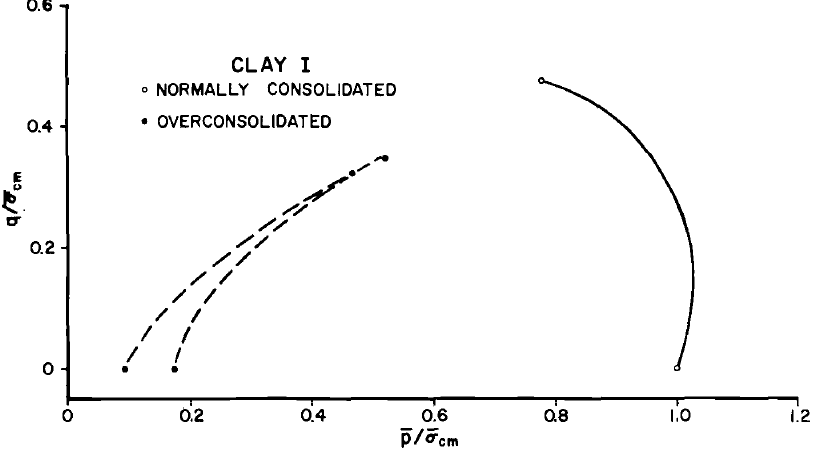
\includegraphics[width=0.48\textwidth]{figures/figure-11a.png}
    }
    \subfigure[EFFECT OF SAMPLING 采样的作用]{
        \label{figure:11b}
        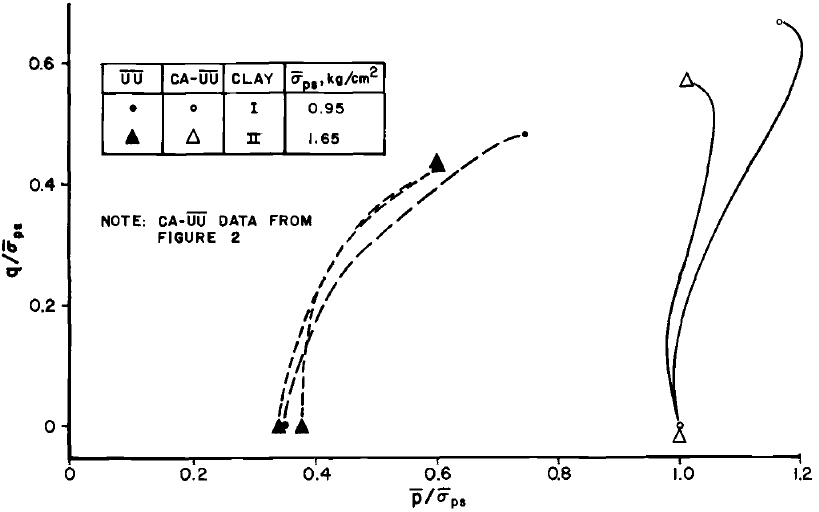
\includegraphics[width=0.48\textwidth]{figures/figure-11b.png}
    }
    \caption{Stress Paths for Kawasaki Clays.}
    \addtocounter{figure}{-1}
    \vspace{-5pt}
    \renewcommand{\figurename}{图}
    \caption{Kawasaki黏土的应力路径。}
    \renewcommand{\figurename}{Figure}
    \label{figure:11}
\end{figure}

\begin{paracol}{2}
    
    This analogy suggests that the strength from UU tests can be considered as test results on overconsolidated specimens with a maximum past pressure equal to $\overline{\sigma}_{ps}$, the value of effective stress existing before gross sample disturbance occurred (see Point P in \autoref{figure:3}). Thus the corrected value of $S_u$ from UU tests, which will correspond to the strength of a specimen after perfect sampling, can be estimated by treating the ratio of $\overline{\sigma}_{ps}$ to $\overline{\sigma}_r$, as an overconsolidation ratio.

    \switchcolumn

    这种类比表明,UU试验的强度可以看作是对超固结试样的试验结果,该试样的最大过去压力等于$\overline{\sigma}_{ps}$,即发生总样本扰动之前存在的有效应力值(参见\cnfigureref{figure:3}中的P点)。 因此,通过将$\overline{\sigma}_{ps}$与$\overline{\sigma}_r$的比值视为过固结率,可以估算出UU试验的$S_u$的校正值,该值对应于完美采样后样品的强度。

    \switchcolumn*

    The proposed method of correcting the undrained shear strength for sample disturbance involves the following three steps: 

    \switchcolumn
   
    校正样品扰动的不排水剪切强度的建议方法包括以下三个步骤:

    \switchcolumn*

    \begin{enumerate}
        \item Relate undrained shear strength to overconsolidation ratio using CIU tests on specimens with $\overline{\sigma}_{cm}$ much greater than $\overline{\sigma}_{v0}$ to reduce the effects of disturbalice, 
        \item Find the equivalent overconsolidation ratio for the UU test being corrected by measuring $\overline{\sigma}_r$ and calculating $\overline{\sigma}_{ps}$, (use \autoref{equation:1} and $CA-\overline{UU}$ data or estimates from \autoref{table:1}), and
        \item Obtain the shear strength correction for the particular overconsolidation ratio as described below.
    \end{enumerate}

    \switchcolumn
    
    \begin{enumerate}
        \item 使用CIU试验对$\overline{\sigma}_{cm}$远大于$\overline{\sigma}_{v0}$的样品考虑不排水剪切强度与超固结率的相关性,以减少干扰的影响,
        \item 通过测量$\overline{\sigma}_r$并计算$\overline{\sigma}_{ps}$,找到要校正的UU试验的等效超固结比(使用\cnequationref{equation:1}和$CA-\overline{UU}$数据或\cntableref{table:1}的估计值),
        \item 获得特定超固结比的抗剪强度修正值,如下面所描述的。
    \end{enumerate}

    \switchcolumn*

    \autoref{figure:12} presents the ratio of undrained shear strength at $\overline{\sigma}_c$ to the strength at $\overline{\sigma}_{cm}$ versus overconsolidation ratio for CIU tests on several natural and remolded clays. As can be seen, the strength ratio decreases significantly with an increase in OCR. Considering the ratio of $\overline{\sigma}_{ps}$ to $\overline{\sigma}_r$ equivalent to OCR, one can read from such a figure the loss in shear strength from excessive sample disturbance which reduces the effective stress from $\overline{\sigma}_{ps}$ to $\overline{\sigma}_r$. From the residual effective stress data already discussed, a typical value of $\overline{\sigma}_r/\overline{\sigma}_{ps}$ might be $\frac{1}{3}$ to $\frac{1}{4}$, the equivalent OCR would then be 3 to 4. Using the data in \autoref{figure:12}, one sees that measured values of UU strength would therefore be 20 to 50 percent too low depending on the type of clay.

    \switchcolumn

    \cnfigureref{figure:12}显示了在几种天然和重塑黏土上进行CIU试验时,$\overline{\sigma}_c$时不排水的剪切强度与$\overline{\sigma}_{cm}$时的强度之比与超固结比。 可以看出,强度比随着OCR的增加而显着降低。 考虑到$\overline{\sigma}_{ps}$与$\overline{\sigma}_r$的比值等于OCR,可以从该图中读取由于过度的样品扰动而导致的剪切强度损失,从而将有效应力从$\overline{\sigma}_{ps}$减小到$\overline{\sigma}_r$。从已经讨论过的残余有效应力数据来看,典型的$\overline{\sigma}_r/\overline{\sigma}_{ps}$值可能是$\frac{1}{3}$到$\frac{1}{4}$,那么等效的OCR就是3到4。使用\cnfigureref{figure:12}中的数据,可以看到,根据黏土的类型,UU强度可能会因此下降20$\%$至50$\%$。

\end{paracol}

\begin{figure}[!htb]
    \centering
    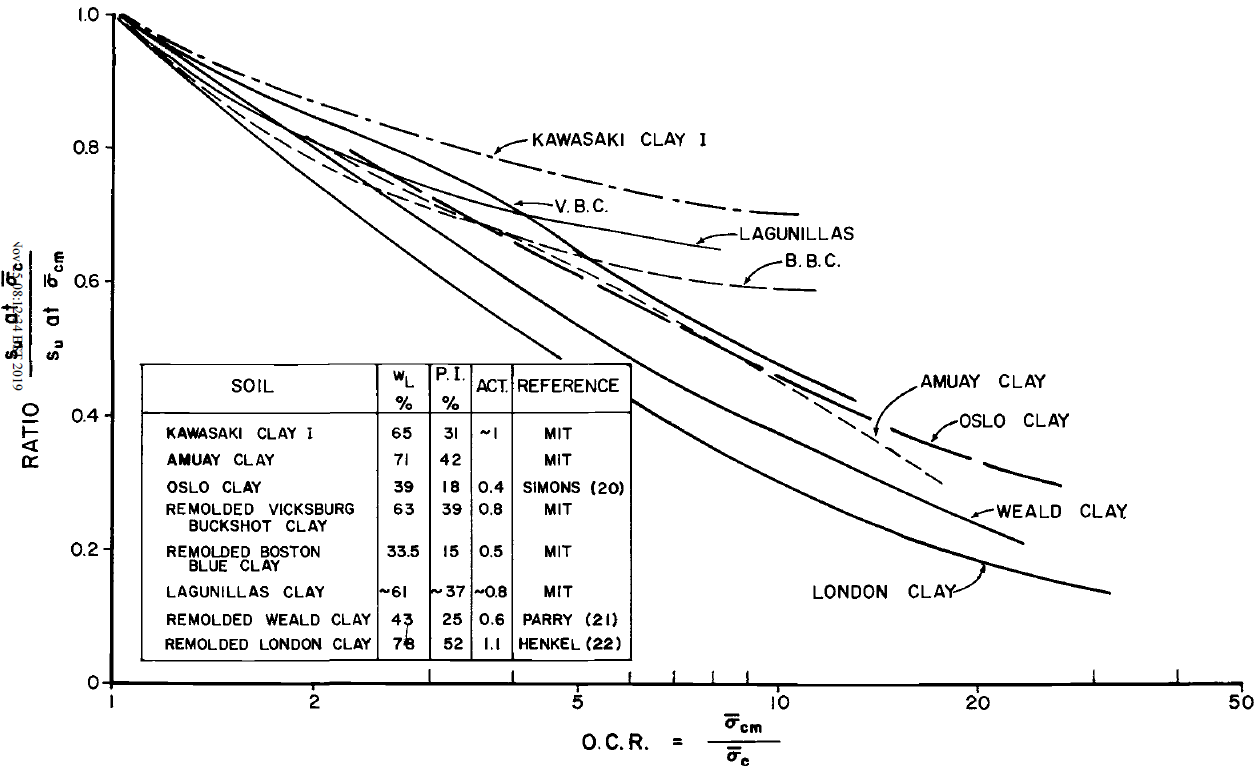
\includegraphics[width=0.7\textwidth]{figures/figure-12.png}
    \caption{Effect of OCR on Undrained Strength.}
    \addtocounter{figure}{-1}
    \vspace{-5pt}
    \renewcommand{\figurename}{图}
    \caption{OCR对不排水强度的影响。}
    \renewcommand{\figurename}{Figure}
    \label{figure:12}
\end{figure}

\begin{paracol}{2}

    Considering a UU test as a test on an overconsolidated specimen is thought to be an important concept. To correct the results of UU tests by use of an equivalent overconsolidation ratio is proposed as an approximate engineering approach. There are both theoretical and practical reasons why such an approach is not precise. Of greatest consequence, it is probably unwarranted to assume with the present state of knowledge that all of the detrimental effects of sampling can be expressed simply as a reduction in effective stress. Further, accurate methods for determining $\overline{\sigma}_{ps}$ are not currently known. Had the specimen existed at a possibly varying $K_0$ effective stress system for a geological time rather than for the time used in the laboratory for a $CA-\overline{UU}$ test, the value of effective stress following perfect sampling might be different. There is also the added problem of the variability in $\overline{\sigma}_r$ measurements. However, to the authors' knowledge, no other method exists for the quantitative evaluation of the very significant effects of disturbance on UU strengths.

    \switchcolumn
        
    将UU试验视为对超固结试样的试验是一个重要的概念。 为了使用等效的超固结比来校正UU试验的结果,建议将其作为一种近似的工程方法。 从理论上和实践上来看,这种方法都不精确。 最重要的结果是,根据目前的知识状况,可能没有必要假设采样的所有有害影响都可以简单地表示为有效压力的降低。 此外,当前没有用于确定$\overline{\sigma}_{ps}$的精确方法。 如果样本存在一个可能变化的$K_0$有效应力系统一段地质时间,而不是在实验室中用于$CA-\overline{UU}$试验的时间,那么完美采样后的有效应力值可能会有所不同。 $\overline{\sigma}_r$测量中的可变性也存在另一个问题。 但是,据作者所知,没有其他方法可以定量评估扰动对UU强度的非常显着的影响。

\end{paracol}
\section{EXAMINATION OF THE CONSOLIDATED-UNDRAINED TEST 固结不排水试验试验}

\begin{paracol}{2}
    
    One widely used technique to estimate the undrained shear strength $S_u$ of an element of clay in the ground is to isotropically consolidate the specimen in the laboratory to a pressure equal to the effective vertical pressure in the ground, and then test the soil in undrained shear. This process involves first a reduction of effective stress and then a reapplication prior to undrained shear. For a normally consolidated specimen, for example, the stresses are reduced from the $K_0$ effective stresses to the isotropic effective stress $\overline{\sigma}_r$, and then reconsolidated isotropically to a stress equal to $\overline{\sigma}_{v0}$. During this large reduction and subsequent increase in effective stresses, and also because of the change from a $K_0$$K_0$ to an isotropic stress system, a significant volume reduction normally occurs. Many (but not all, such as \citet{Taylor1948}, p.397) soil engineers feel that this volume decrease results in an undrained shear strength which is too large. For example, see \citet{Rutledge19441155}, p.1216, \citet{Hansen1948189}, p.204, \citet{Osterberg1956}, p.70, and \citet{Bishop1960437}, p.449.

    \switchcolumn

    估算地面中黏土元素的不排水抗剪强度$S_u$的一种广泛使用的技术是在实验室中将试样各向同性地固结到等于地面中有效垂直压力的压力,然后对其进行不排水的剪切试验。该过程首先涉及减小有效应力,然后在不排水剪切之前重新施加应力。 例如,对于正常固结的试样,应力从$K_0$有效应力减小到各向同性有效应力$\overline{\sigma}_r$,然后各向同性地再固结到等于$\overline{\sigma}_{v0}$的应力。 在这种较大的减小和随后的有效应力增加期间,并且还由于从$K_0$变为各向同性应力系统,通常会发生明显的体积减小。 许多岩土工程师(但不是全部,例如\citet{Taylor1948}第397页)认为,这种体积减小会导致不排水的剪切强度过大。 例如,请参见\citet{Rutledge19441155}第1216页,\citet{Hansen1948189}第204页,\citet{Osterberg1956}第70页以及\citet{Bishop1960437}第449页。

\end{paracol}

\Paragraph{Published Methods of Correcting CIU Test Results: 修正CIU试验结果的已有方法:}

\begin{paracol}{2}
    
    Several methods have been suggested for evaluating the effects of volume change on undrained strength. These methods generally extrapolate, in various ways, a plot of $\log{}S_u$ from CIU triaxial tests versus void ratio $e$ to a value of $S_u$ corresponding to the in-situ void ratio. For example, \citet{Schmertmann1956940} draws a line through the point of intersection of lines of $\log{}S_u-e$ for CIU tests on undisturbed and remolded specimens and parallel to the estimated slope of the in situ consolidation curve. The intersection of this line with the in-situ void ratio yields the field undisturbed strength. \citet{Calhoon1956925} shifts the plot of log s versus e from CIU triaxial tests upward in proportion to the per cent disturbance of the triaxial specimens. The percent disturbance is deduced from the location of the $\log{}S_u-e$ curve from the triaxial tests in relationship to $\log{}S_u-e$ plots from oedometer tests on varying size specimens and on a remolded specimen.\footnote{
        This method assumes that only trimming produces sample disturbance, which can be very incorrect, and it neglects the effect of K on the location of c curves. 该方法假定仅对样品的修剪会产生样本干扰,这可能是非常不正确的,并且忽略了K对$\overline{\sigma}_c$曲线位置的影响。} 
    One of the simplest methods, that of \citet{Casagrande1947}, as quoted by \citet{Hvorslev1949}, suggests an extrapolation of the $\log{}S_u-e$ line from CIU tests back to the in situ void ratio as an approximate approach for obtaining $S_u$ corresponding to no volume change.

    \switchcolumn

    已经提出了几种方法来评估体积变化对不排水强度的影响。 这些方法通常以各种方式将来自CIU三轴试验的$\log{}S_u$与孔隙率$e$的关系图推导出对应于原位孔隙率的$S_u$值。 例如,\citet{Schmertmann1956940}在原状和重塑试样上进行CIU试验时,通过$\log{}S_u-e$曲线的交点画一条线,该线平行于原位固结曲线的估计斜率。 这条线与原位空隙率的交点产生了不受干扰的场强。\footnote{Need to change}\citet{Calhoon1956925}将CIU三轴试验的$\log{}S_u-e$的曲线与三轴试样的扰动百分比成比例地向上移动。 干扰百分比从三轴试验中的$\log{}S_u-e$曲线和不同尺寸的样品和重塑的样品上的固结试验得到的$\log{}S_u-e$图的位置关系中得出。\footnote{Need to change} 最简单的方法之一,如\citet{Hvorslev1949}所引用的\citet{Casagrande1947}的方法,建议将CIU试验的$\log{}S_u-e$曲线外推到原位空隙率作为获得对应于无体积变化的$S_u$的近似方法。

    \switchcolumn*

    The application of these methods to the strength data on Kawasaki Clay I, \autoref{figure:10}, yielded the values of $S_u$ corrected for volume change,\footnote{
        There are insufficient data on the other cases in \autoref{table:2} to allow similar analyses. \cntableref{table:2}中其他案例的数据不足,无法进行类似的分析。
    } shown in \autoref{table:3}. There is a wide divergence in the resulting strengths. Two of the methods yielded strengths which are too low since they are equal to, or smaller than, the 0.5 $\rm{kg/cm^2}$ from the UU tests. On the other hand, the $S_u$ from the Calhoon method is too high since CIU tests with $\overline{\sigma}_c=\overline{\sigma}_{v0}$ yielded an $S_u$ of only about 0.8 $\rm{kg/cm^2}$ (\autoref{figure:8}). Even if the Kawasaki Clay I represents an unusual case, these methods would appear to be questionable.

    \switchcolumn

    将这些方法应用于\cnfigureref{figure:10}所示的Kawasaki黏土I的强度数据后,得出的$S_u$值已针对体积变化进行了修正,如\cntableref{table:3}所示。在结果上存在很大差异。 两种方法得出的强度太低,因为它们等于或小于UU试验中的0.5$\rm{kg/cm^2}$。 另一方面,来自Calhoon方法的$S_u$太大,因为$\overline{\sigma}_c=\overline{\sigma}_{v0}$时的CIU试验得出的$S_u$仅为0.8$\rm{kg/cm^2}$(\cnfigureref{figure:8})。即使Kawasaki黏土I代表一个不寻常的情况,这些方法似乎仍然值得怀疑。

\end{paracol}

\begin{table}[!htb]
    \centering
    \caption{PREDICTION OF UNDRAINED STRENGTH AT IN SITU VOID RATIO FROM CIU TRIAXIAL TESTS BY PREVIOUS METHODS FOR KAWASAKI CLAY I.}
    \addtocounter{table}{-1}
    \vspace{-8pt}
    \renewcommand{\tablename}{表}
    \caption{川崎黏土I的先前方法从CIU三轴试验预测原位空隙率的不排水强度。}
    \vspace{4pt}
    \renewcommand{\tablename}{Table}
    \begin{threeparttable}[b]
        \begin{tabularx}{\textwidth}{ll}
            \toprule
            Method & $S_u{\rm (kg/cm^2)~for}~ \Delta{}e/(1+e_0)=0$\\
            \midrule
            \citet{Schmertmann1956940} & ~~0.3 to 0.45 \\
            \citet{Calhoon1956925} & $\sim$0.85 \\
            \citet{Casagrande1947} & $\sim$0.5 \\
            Average of unconfined\tnote{a} compression tests & ~~0.45\tnote{b} \\
            Average of $\overline{UU}$ and top one third of unconfined compression tests & ~~0.5\tnote{b} \\
            \bottomrule
        \end{tabularx}%
        \begin{tablenotes}
            \item[a] Many of the specimens contained lenses of sand, silt, or shells which caused very low unconfined strengths. 许多标本包含沙粒,粉尘或贝壳状的透镜,这些透镜的强度很低。
            \item[b] Corrected to correspond to $t_f=5$ hr. 校正为对应于 $t_f=5$小时。
        \end{tablenotes}
    \end{threeparttable}
    \label{table:3}%
\end{table}


\Paragraph{Proposed Methods of Correcting CIU Test Results: 修正CIU试验结果的建议方法:}

\begin{paracol}{2}

    One way to account for the effects on $S_u$ of the volume change upon reconsolidation is to use the Hvorslev \citet{Hvorslev1960169}, p. 210 or \citet{Bishop1962}, p. 166 which can be expressed as follows: $\big(\dfrac{1}{2}(\sigma_1-\sigma_3)_f$ is replaced by $S_u$ since only undrained shear strength is considered$\big)$

    \switchcolumn

    解决固结对体积变化$S_u$的影响的一种方法是使用Hvorslev参数\citet{Hvorslev1960169}第210页或\citet{Bishop1962}第166页,可以表示为:$\big(\dfrac{1}{2}(\sigma_1-\sigma_3)_f$被$S_u$代替,因为只考虑了不排水的剪切强度$\big)$

\end{paracol}

\begin{align}
    S_u=H\overline{\sigma}_e+\overline{\sigma}_{3f}\tan\overline{\theta}_e
    \label{equation:2}
\end{align}

\begin{paracol}{2}

    \noindent{}where:\\
    \newlength\length
    \settowidth{\length}{$\tan\overline{\theta}_e$}
    \makebox[\length][l]{H} = $K(\cos\overline{\phi}_e)/(1-\sin\overline{\phi}_e)$, \\
    \makebox[\length][l]{$\tan\overline{\theta}_e$} = $(\sin\overline{\phi}_e)/(1-\sin\overline{\phi}_e)$, \\
    \makebox[\length][l]{K} = $\overline{c}_e/\overline{\sigma}_e$, \\
    \makebox[\length][l]{$\overline{c}_e$} = Hvorslev cohesion, \\
    \makebox[\length][l]{$\overline{\phi}_e$} = Hvorslev friction angle, and \\
    \makebox[\length][l]{$\overline{\sigma}_e$} = Hvorslev equivalent consolidation pressure. 

    \switchcolumn

    \noindent{}式中:\\
    \makebox[\length][l]{H} = $K(\cos\overline{\phi}_e)/(1-\sin\overline{\phi}_e)$, \\
    \makebox[\length][l]{$\tan\overline{\theta}_e$} = $(\sin\overline{\phi}_e)/(1-\sin\overline{\phi}_e)$,\\
    \makebox[\length][l]{K} = $\overline{c}_e/\overline{\sigma}_e$, \\
    \makebox[\length][l]{$\overline{c}_e$} = Hvorslev粘聚力, \\
    \makebox[\length][l]{$\overline{\phi}_e$} = Hvorslev摩擦角,以及 \\
    \makebox[\length][l]{$\overline{\sigma}_e$} = Hvorslev等效固结压力。

    \switchcolumn*

    \noindent{}If two specimens were consolidated to the same pressure, but had different water contents and hence different values of $\overline{\sigma}_e$, then the difference in $S_u$ for undrained shear could be reflected in changes in both $H\overline{\sigma}_e$ and $\overline{\sigma}_{3f}\tan\overline{\theta}_e$. However, if $\overline{\sigma}_{3f}$ were independent of the water content change, the difference in $S_u$ could be calculated from the change in $H\overline{\sigma}_e$, assuming of course, that H and $H\overline{\theta}_e$ were constants for the soil.\footnote{
        \citet{Bjerrum1960101} show that H varies with consolidation pressure for undisturbed specimens of Lilla Edet clay, which is believed to have a significant amount of natural eementation. \citet{Bjerrum1960101}表明,对于Lilla Edet黏土的未扰动标本,H随固结压力的变化而变化,该黏土被认为具有大量的自然胶结作用。
    }

    \switchcolumn

    \noindent{}如果将两个试样固结到相同的压力下,但是含水量不同,因此$\overline{\sigma}_e$值也不同,则不排水剪切的$S_u$差异可以反映在$H\overline{\sigma}_e$和$\overline{\sigma}_{3f}\tan\overline{\theta}_e$的变化中。但是,如果$\overline{\sigma}_{3f}$与含水量的变化无关,则可以根据$H\overline{\sigma}_e$的变化来计算$S_u$的差,当然,假设H和$H\overline{\theta}_e$是土体的常数。

\end{paracol}
    
\begin{figure}[!htbp]
    \centering
    \begin{minipage}[t]{0.48\textwidth}
        \centering
        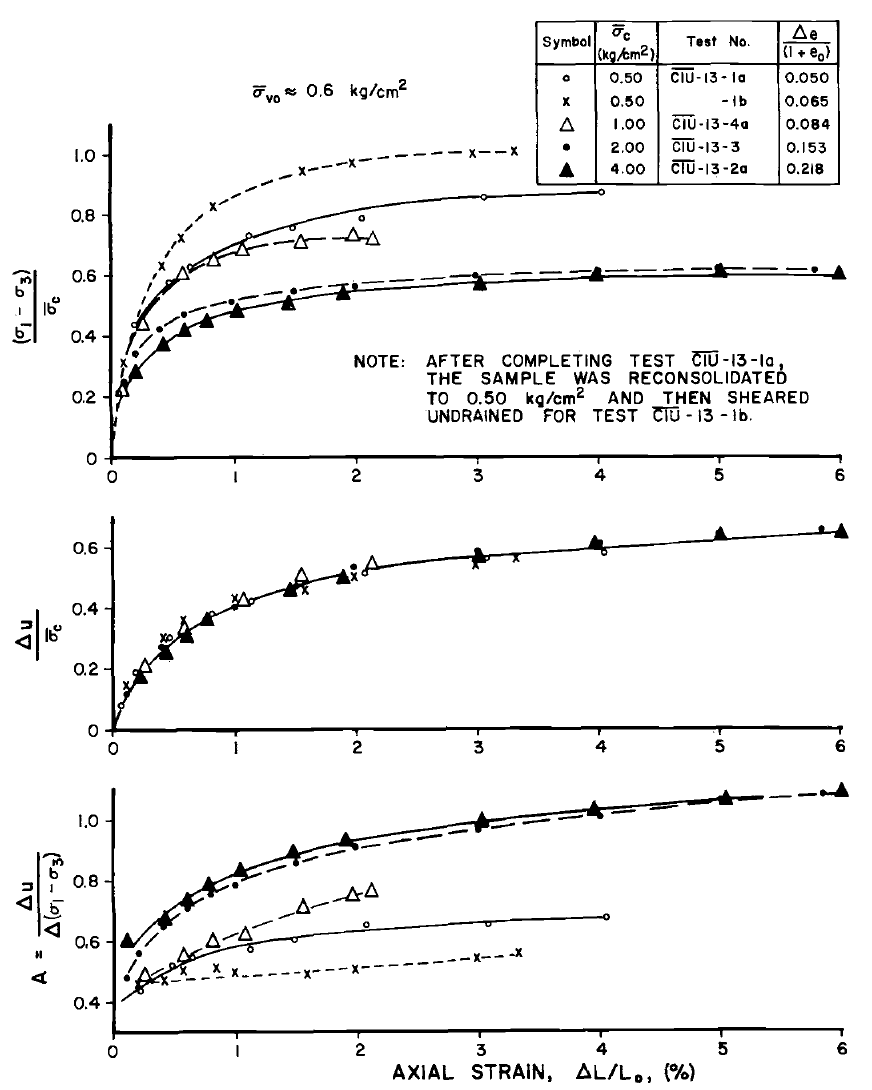
\includegraphics[width=0.9\textwidth]{figures/figure-13.png}
        \caption{Effect of Consolidation Pressure and Reconsolidation on the Stress-Strain Behavior of Lagunillas Clay.}
        \vspace{-5pt}
        \addtocounter{figure}{-1}
        \renewcommand{\figurename}{图}
        \caption{固结压力和再固结对Lagunillas黏土应力应变行为的影响。}
        \label{figure:13}
        \renewcommand{\figurename}{Figure}
    \end{minipage}
    \begin{minipage}[t]{0.48\textwidth}
        \centering
        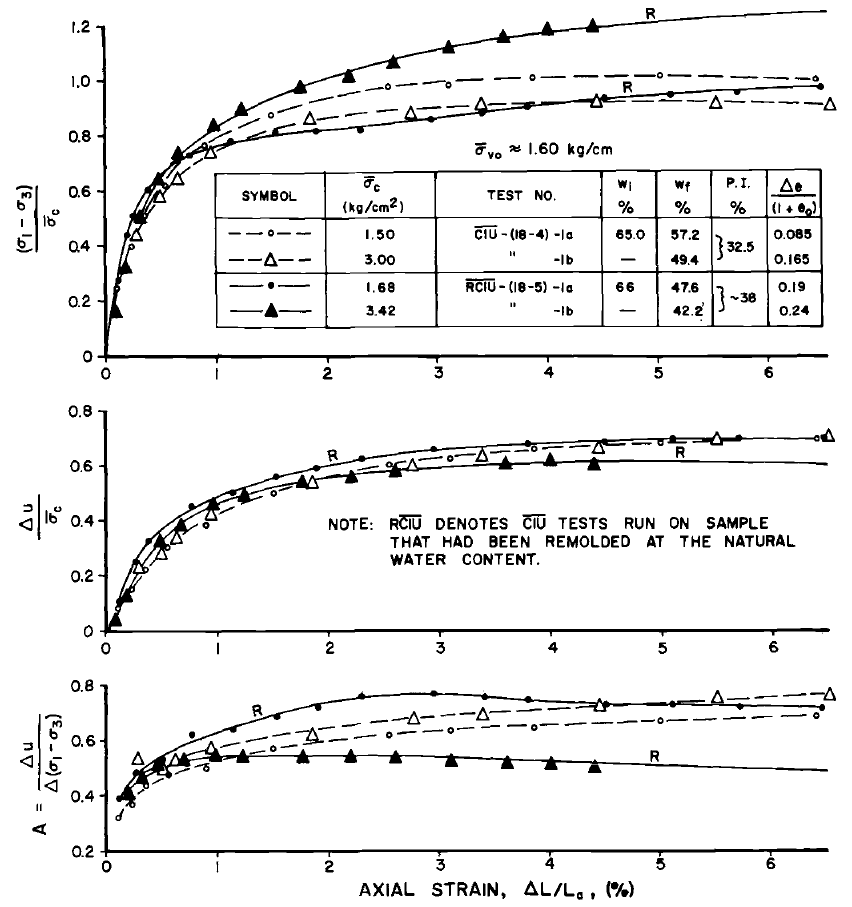
\includegraphics[width=0.9\textwidth]{figures/figure-14.png}
        \caption{Effect of Consolidation Pressure and Remolding on the Stress-Strain Behavior of Kawasaki Clay I.}
        \vspace{-5pt}
        \addtocounter{figure}{-1}
        \renewcommand{\figurename}{图}
        \caption{固结压力和重塑对Kawasaki黏土I应力-应变行为的影响。}
        \label{figure:14}
        \renewcommand{\figurename}{Figure}
    \end{minipage}
\end{figure}

\begin{paracol}{2}

    Since $\overline{\sigma}_{3f}$ is directly related to the excess pore pressure at failure, one can look at the effects of volume change on the pore pressure behavior of $\overline{CIU}$ tests. Such data for the Lagunillas clay and the Kawasaki Clay I are presented in \autoref{figure:13} and \autoref{figure:14}. The data show that $\Delta{}u/\overline{\sigma}_c$ versus strain is practically independent of (1) consolidation pressure for $\overline{\sigma}_c$ values greater than $\overline{\sigma}_{ps}$, even though the value of volumetric strain compared to the in situ value varies considerably with consolidation pressure (\autoref{figure:9} and \autoref{figure:10}), (2) reconsolidation, with resultant volume decrease, after undrained shear (Test $\overline{CIU}-13-1(b)$ in \autoref{figure:13}), and (3) remolding at the natural water content with subsequent consolidation and very large volume changes (Tests $R\overline{CIU}-(18-5)-1(a)$ and $-1(b)$ in \autoref{figure:14}). As a reasonable approximation it is therefore assumed that the volume change caused by the consolidation of $\overline{CIU}$ specimens to pressures between $\overline{\sigma}_{ps}$ and $\overline{\sigma}_{v0}$ has little effect on $\Delta{}u/\overline{\sigma}_c$ during undrained shear, and that the strain at failure is also unaltered. The decrease in $S_u$ is then calculated from the change in Hvorslev cohesion, $H\Delta{}\overline{\sigma}_e$, commensurate with the decrease in volume from the in situ condition, $\Delta{}e/(1+e_0)$. An example is given in the next section.

    \switchcolumn

    由于$\overline{\sigma}_{3f}$与失效时多余的孔隙压力直接相关,因此可以查看体积变化对$\overline{CIU}$试验的孔隙压力行为的影响。Lagunillas黏土和Kawasaki黏土I的这些数据在\cnfigureref{figure:13}和\cnfigureref{figure:14}显示。数据显示$\Delta{}u/\overline{\sigma}_c$与应变的关系实际上与(1)超过$\overline{\sigma}_{ps}$的$\overline{\sigma}_c$值的固结压力,即使体积应变的值与原位试验值相比随固结压力变化很大(\cnfigureref{figure:9}和\cnfigureref{figure:10}),(2)在不排水的剪切之后重新固结,导致体积减小(\cnfigureref{figure:13}中的试验$\overline{CIU}-13-1(b)$)以及(3)在天然含水量下重塑并随后固结以及非常大的体积变化(\cnfigureref{figure:14}中的$R\overline{CIU}-(18-5)-1(a)$和$-1(b)$试验)无关。因此,作为合理的近似值,可以假设在不排水的剪切过程中,在固结应力为$\overline{\sigma}_{ps}$和$\overline{\sigma}_{v0}$之间时,由$\overline{CIU}$试样的固结引起的体积变化对$\Delta{}u/\overline{\sigma}_c$的影响很小,并且破坏时的应变也没有改变。$S_u$的减少可通过Hvorslev内聚力$H\Delta{}\overline{\sigma}_e$的变化与原位条件下体积的减少$\Delta{}e/(1+e_0)$相称来计算。下一节将给出一个示例。

    \switchcolumn*

    Another possible approach to the problem of assessing the effects of volume change would be to use the results of CU tests at consolidation pressures much larger than $\overline{\sigma}_{v0}$, where the effects of specimen disturbance might be minimized \citet{Marsal1957229}, p. 194, \citet{Casagrande1953}, p. 33. This method, as with previous ones, requires negligible changes in soil structure with consolidation pressure. If the value of $S_u$ corresponding to perfect sampling is desired, CA-UU tests should be used with consolidation pressures at least two to four times $\overline{\sigma}_{v0}$.

    \switchcolumn

    评估体积变化影响的另一种可能的方法是,在固结压力远大于$\overline{\sigma}_{v0}$的情况下使用CU试验的结果,在这种情况下,样品扰动的影响可能会最小化\citet{Marsal1957229}第194页,\citet{Casagrande1953}第33页。与以前一样,这种方法要求土壤结构随固结压力的变化可忽略不计。 如果需要与完美采样相对应的$S_u$值,则应使用固结压力至少为$\overline{\sigma}_{v0}$的2-4倍的CA-UU试验。

\end{paracol}
\section{COMPARISON OF CORRECTED UU AND CU TEST RESULTS 修正的UU和CU试验结果的比较}

\Paragraph{Results for Kawasaki and Lagunillas Clays: Kawasaki和Lagunillas黏土的结果:}

\begin{paracol}{2}
    
    Specific examples illustrating the application of the authors' methods of correcting UU and CU test data for sample disturbance will be presented first. In reiteration, the primary objective of the correction is to arrive at an undrained shear strength for triaxial compression of a specimen subjected to perfect sampling, that is, the specimen had a preshear effective stress equal to $\overline{\sigma}_{ps}$ (\autoref{equation:1}) and the in-situ void ratio. Test data for Kawasaki Clay I will be used for the illustrative examples.

    \switchcolumn

    首先将给出具体示例,这些示例说明作者针对样本干扰校正UU和CU试验数据的方法的应用。 重申一下,校正的主要目的是在经受完美采样的样品上获得不排水的剪切强度,以进行三轴压缩,也就是说,样品有一个预剪切有效应力等于$\overline{\sigma}_{ps}$(\cnequationref{equation:1})和原位空隙率。 Kawasaki黏土I的试验数据将用于说明示例。

    \switchcolumn*

    \emph{Correction of UU Data for Test $\overline{UU}-(18-5)-1$} (strain rate effects will be neglected).

    \switchcolumn

    \emph{对试验$\overline{UU}-(18-5)-1$的UU数据进行校正}(应变率影响将被忽略)。
  
    \switchcolumn*

    1. Measured data (\autoref{figure:6}): $S_u=0.46{\rm kg/cm^2}$ and $\overline{\sigma}_r=0.34{\rm kg/cm^2}$.

    2. Equivalent OCR (\autoref{figure:4}): Since specimen depth was 21.2 m, $\overline{\sigma}_{ps}=0.95{\rm kg/cm^2}$. Therefore, the equivalent ${\rm OCR}=\overline{\sigma}_{ps}/\overline{\sigma}_r=0.46/0.82=0.56{\rm kg/cm^2}$.

    3. Corrected strength: For an OCR=2.80, and using \autoref{figure:12}, $S_u~{\rm at}~\overline{\sigma}_c/S_u~{\rm at}~\overline{\sigma}_{cm}=0.82$. Since this ratio is also assumed equal to $S_u~{\rm at}~\overline{\sigma}_r/S_u~{\rm at}~\overline{\sigma}_{ps}$, the corrected $S_u=0.46/0.82=0.56{\rm kg/cm^2}$.

    \switchcolumn

    1.实测数据(\cnfigureref{figure:6}):$S_u=0.46{\rm kg/cm^2}$,$\overline{\sigma}_r=0.34{\rm kg/cm^2}$。
    
    2.等效OCR(\cnfigureref{figure:4}):由于样品深度为21.2 m,$\overline{\sigma}_{ps}=0.95{\rm kg/cm^2}$。因此,等效${\rm OCR}=\overline{\sigma}_{ps}/\overline{\sigma}_r=0.46/0.82=0.56{\rm kg/cm^2}$。
   
    3.校正强度:对于OCR=2.80,并使用\cnfigureref{figure:12},$S_u~{\rm at}~\overline{\sigma}_c/S_u~{\rm at}~\overline{\sigma}_{cm}=0.82$。 由于还假定该比率等于$S_u~{\rm at}~\overline{\sigma}_r/S_u~{\rm at}~\overline{\sigma}_{ps}$,因此校正后的$S_u=0.46/0.82=0.56{\rm kg/cm^2}$。

\end{paracol}

\Paragraph{Correction of CU Data for Depth of 23 M: CU数据深度为23米的校正:}

\begin{paracol}{2}

    \emph{1. Hvorslev parameters:} Values of the Hvorslev parameters are shown in \autoref{figure:15} for both the Lagunillas clay and Kawasaki Clay I where $\overline{\sigma}_e$, was based on values of $\Delta{e}/(1+e_0)$ in \autoref{figure:9} and \autoref{figure:10} rather than water content, which varied erratically. The parameters were determined on the basis of $\overline{CU}$ and \emph{CID} tests, although $\overline{UU}$ and $\overline{RCIU}$ test data have been added for interest.

    \switchcolumn

    \emph{1. Hvorslev参数:}Lagunillas黏土和Kawasaki黏土I的Hvorslev参数值如\cnfigureref{figure:15}所示,其中$\overline{\sigma}_e$是基于\cnfigureref{figure:9}和\cnfigureref{figure:10}中的$\Delta{e}/(1+e_0)$值,而不是水含量,这是不规则的变化。 尽管已添加了$\overline{UU}$和$\overline{RCIU}$试验数据,但这些参数是根据$\overline{CU}$和\emph{CID}试验确定的。

\end{paracol}

\begin{figure}[!htbp]
    \centering
    \subfigure[Kawasaki Clays I]{
        \label{figure:15a}
        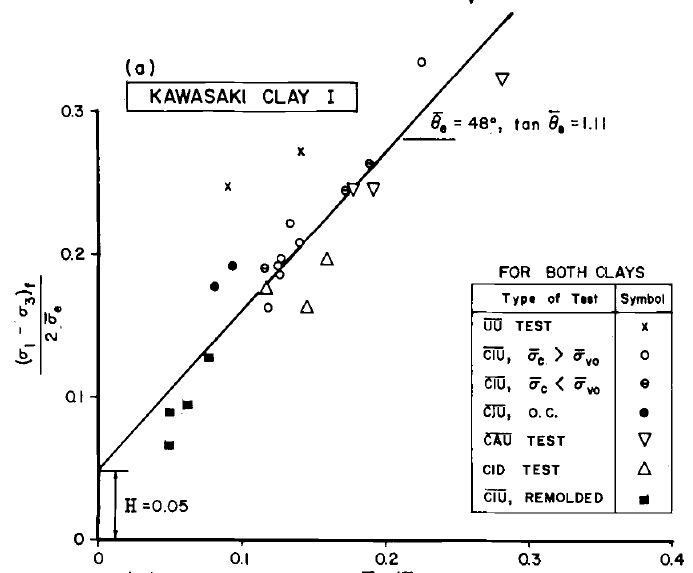
\includegraphics[width=0.48\textwidth]{figures/figure-15a.png}
    }
    \subfigure[Lagunilla Clay]{
        \label{figure:15b}
        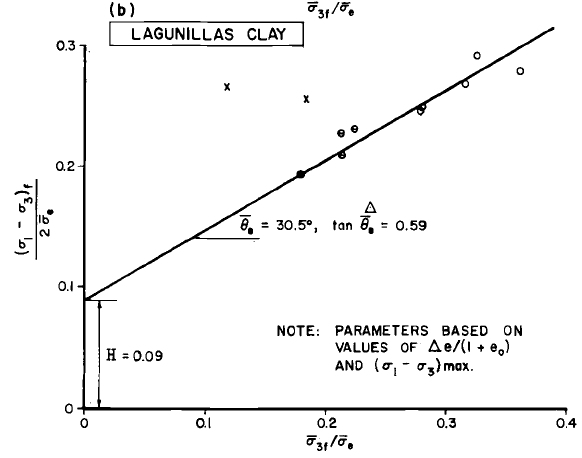
\includegraphics[width=0.48\textwidth]{figures/figure-15b.png}
    }
    \caption{Hvorslev Parameters.}
    \addtocounter{figure}{-1}
    \vspace{-5pt}
    \renewcommand{\figurename}{图}
    \caption{Hvorslev参数}
    \renewcommand{\figurename}{Figure}
    \label{figure:15}
\end{figure}
\begin{sidewaystable}[p]
    \centering
    \footnotesize
    \caption{COMPARISON OF CORRECTED UNDRAINED STRENGTH FROM UU AND CU TESTS ON NORMALLY CONSOLIDATED KAWASAKI AND LAGUNILLAS CLAYS.}
    \addtocounter{table}{-1}
    \vspace{-8pt}
    \renewcommand{\tablename}{表}
    \caption{正常固结的Kawasaki和Lagunillas黏土上UU和CU试验的修正不排水强度的比较。}
    \vspace{4pt}
    \renewcommand{\tablename}{Table}
    \begin{threeparttable}
    \setlength{\tabcolsep}{1.0mm}{
        \begin{tabular}{llllllllllllllll}
            \toprule
            \multirow{3}{*}{Location}        & \multirow{3}{*}{Clay} & \multirowcell{3}[1pt][l]{Depth,\\m} & \multirowcell{3}[1pt][l]{$\overline{\sigma}_{v0}$,\\$\rm{kg/cm^2}$} & \multirowcell{3}[1pt][l]{$\overline{\sigma}_{ps}$,\\$\rm{kg/cm^2}$} & \multicolumn{2}{l}{\multirowcell{2}[1pt][l]{$S_u/\overline{\sigma}_{v0}$ From \\UU Tests}} & \multicolumn{4}{l}{$S_u/\overline{\sigma}_{v0}$ From CIU Tests}                          & \multicolumn{2}{l}{\multirowcell{2}[1pt][l]{Measured\tnote{c}\\$\frac{S_u(UU)}{S_u(CIU)}$}} & \multicolumn{2}{l}{\multirowcell{2}[1pt][l]{Corrected\tnote{d}\\$\frac{S_u(UU)}{S_u(CIU)}$}} & \multirowcell{3}[1pt][l]{$\frac{S_u(UU)}{S_u(CIU)}$\tnote{e}\\$S_u(CU)$ from\\$CA-\overline{UU}$ Tests\\(11)} \\
                                             &                       &                          &                        &                        & \multicolumn{2}{l}{}                                 & \multicolumn{2}{l}{Measured\tnote{a}} & \multicolumn{2}{l}{Corrected\tnote{b}} & \multicolumn{2}{l}{}                          & \multicolumn{2}{l}{}                           &                     \\
                                             &                       &                          &                        &                        & \makecell[l]{Measured\\(1)}                 & \makecell[l]{Corrected\tnote{f}\\(2)}                 & \makecell[l]{$\overline{\sigma}_c=\overline{\sigma}_{v0}$\\(3)}             & \makecell[l]{$\overline{\sigma}_c=\overline{\sigma}_{ps}$\\(4)}            & \makecell[l]{$\overline{\sigma}_c=\overline{\sigma}_{v0}$\\(5)}             & \makecell[l]{$\overline{\sigma}_c=\overline{\sigma}_{ps}$\\(6)}             & \makecell[l]{$\overline{\sigma}_c=\overline{\sigma}_{v0}$\\(7)}                     & \makecell[l]{$\overline{\sigma}_c=\overline{\sigma}_{ps}$\\(8)}                     & \makecell[l]{$\overline{\sigma}_c=\overline{\sigma}_{v0}$\\(9)}                      & \makecell[l]{$\overline{\sigma}_c=\overline{\sigma}_{ps}$\\(10)}                     &                     \\
            \midrule
            \multirowcell{2}[1pt][l]{Kawasaki, \\~~Japan} & \multirowcell{2}[11pt][l]{Clay I,P.I.=31$\%$\\Clay I,P.I.=36$\%$\\Clay II,P.I.=43$\%$} &  \makecell[l]{20.5\\25\\36}                        & \makecell[l]{1.60\\1.88\\2.62}                       & \makecell[l]{0.92\\1.08\\1.64}                       & \makecell[l]{0.31\tnote{g}\\0.26\tnote{g}\\0.27\tnote{g}}                         & \makecell[l]{0.38\\0.32\\0.33}                          & \makecell[l]{0.485\\0.45\\0.475}              & \makecell[l]{0.42\\0.37\\0.36}             & \makecell[l]{0.43\\0.395\\0.42}              & \makecell[l]{0.40\\0.35\\0.335}              & \makecell[l]{0.64\\0.58\\0.57}                      & \makecell[l]{0.74\\0.70\\0.75}                      & \makecell[l]{0.88\\0.81\\0.78}                       & \makecell[l]{0.95\\0.91\\0.98}                      & \makecell[l]{1.12\\0.89\\1.00}                    \\
                                             &                       & \multicolumn{9}{l}{Average}                                                                                                                                                                      &  0.59                     & 0.73                      & 0.82                       & 0.95                      & 1.00                    \\
            \makecell[l]{Lagunillas, \\~~Venezuela}            & \makecell[l]{plastic clay,\\~~~~P.I.=37$\%$}   & 6.4                         & 0.62                       & \makecell[l]{0.40\\(Estimated)}                       & 0.255\tnote{h}                         & 0.345                          & 0.40              & 0.335             & 0.38              & 0.325              & 0.64                      & 0.77                      &  0.91                      & 1.05                      & $\cdots$                    \\
            \bottomrule
        \end{tabular}}%
        \begin{tablenotes}
            \item[a] From \autoref{figure:7} and \autoref{figure:8} or similar data. $\overline{\sigma}_c=\overline{\sigma}_{v0}$ means that $S_u$ is taken at $\overline{\sigma}_c=\overline{\sigma}_{v0}$; for $\overline{\sigma}_c=\overline{\sigma}_{ps}$, $S_u$ is taken at $\overline{\sigma}_c=\overline{\sigma}_{v0}$. 来自\cnfigureref{figure:7}和\cnfigureref{figure:8}或类似数据。$\overline{\sigma}_c=\overline{\sigma}_{v0}$代表$S_u$在$\overline{\sigma}_c=\overline{\sigma}_{v0}$时获得,$\overline{\sigma}_c=\overline{\sigma}_{ps}$代表$S_u$在$\overline{\sigma}_c=\overline{\sigma}_{ps}$时获得。
            \item[b] Based on Hvorslev parameters. That is, $\Delta{S_u}=H\Delta{\overline{\sigma}_e}$. 基于Hvorslev参数,即$\Delta{S_u}=H\Delta{\overline{\sigma}_e}$。
            \item[c] Columns (1) over (3) and (1) over (4) respectively. 分别对应于列1/列3和列1/列4。
            \item[d] Columns (2) over (5) and (2) over (6) respectively. 分别对应于列2/列5和列2/列6。
            \item[e] $S_u(CU)$ from $S_u/\overline{\sigma}_{1c}$ ratio from $CA-\overline{UU}$ tests at $\overline{\sigma}_{1c}$ values 2-4 times $s_u/\overline{\sigma}_{v0}$ from Column 2. 来自$CA-\overline{UU}$试验的$S_u/\overline{\sigma}_{1c}$的$S_u(CU)$在数值上时列2中$s_u/\overline{\sigma}_{v0}$的2-4倍。
            \item[f] Correction for Kawasaki based on taking O.C.R. = 2.85 ($\overline{\sigma}_r/\overline{\sigma}_{ps}=0.35$ which corresponds to values for the better samples). Correction for Lagunillas based on taking O.C.R. = 2.8 ($\overline{\sigma}_r/\overline{\sigma}_{ps}=0.36$). 根据O.C.R. = 2.85对Kawasaki的修正($\overline{\sigma}_r/\overline{\sigma}_{ps}=0.35$,对应于较好样本的值)。 根据O.C.R.修正Lagunillas  = 2.8($\overline{\sigma}_r/\overline{\sigma}_{ps}=0.35$)。
            \item[g] Average from UU and top one-third of U tests corrected to $t_f$ = 5 hr. UU和U试验的前三分之一的平均值已校正为$t_f$ = 5小时。
            \item[h] Average from UU tests for which ~r measurements available. 如果$\overline{\sigma}_r$可测量时UU试验的平均值。
        \end{tablenotes}
    \end{threeparttable}
    \label{table:4}%
\end{sidewaystable}


\begin{paracol}{2}
    
    \emph{2. Measured data:} For a depth of 23m \autoref{figure:4} shows that $\overline{\sigma}_{v0}=1.75{\rm kg/cm^2}$ and $\overline{\sigma}_{ps}=1.00{\rm kg/cm^2}$. From \autoref{figure:8} at $\overline{\sigma}_c=\overline{\sigma}_{ps}=1.00{\rm kg/cm^2}$, the measured $S_u=0.68{\rm kg/cm^2}$. For $\overline{\sigma}_c=1.00{\rm kg/cm^2}$, a representative value of $\Delta{e}/(1+e_0)=0.04$ from \autoref{figure:10}.

    \switchcolumn

    \emph{2.测量数据:}对于23m的深度,\cnfigureref{figure:4}表明$\overline{\sigma}_{v0}=1.75{\rm kg/cm^2}$,$\overline{\sigma}_{ps}=1.00{\rm kg/cm^2}$。\cnfigureref{figure:8}的$\overline{\sigma}_c=\overline{\sigma}_{ps}=1.00{\rm kg/cm^2}$,实测值$S_u=0.68{\rm kg/cm^2}$。 对于$\overline{\sigma}_c=1.00{\rm kg/cm^2}$,\cnfigureref{figure:10}的代表值$\Delta{e}/(1+e_0)=0.04$。

    \switchcolumn*

   \emph{3. Equivalent consolidation pressures} (\autoref{figure:10}): For $\Delta{e}/(1+e_0)=0.04$, $\overline{\sigma}_e=2.60{\rm kg/cm^2}$; this represents isotropic consolidation of a lab specimen to $\overline{\sigma}_c=\overline{\sigma}_{ps}=1.00{\rm kg/cm^2}$. For perfect sampling, $\Delta{e}/(1+e_0)=0$ and $\overline{\sigma}_e=\overline{\sigma}_{v0}=1.75{\rm kg/cm^2}$.

    \switchcolumn

    \emph{3.当量固结压力}(\cnfigureref{figure:10}):对于$\Delta{e}/(1+e_0)=0.04$,$\overline{\sigma}_e=2.60{\rm kg/cm^2}$;这表示实验室样品的各向同性固结至$\overline{\sigma}_c=\overline{\sigma}_{ps}=1.00{\rm kg/cm^2}$。 对于完美采样,$\Delta{e}/(1+e_0)=0$且$\overline{\sigma}_e=\overline{\sigma}_{v0}=1.75{\rm kg/cm^2}$。

    \switchcolumn*

    \emph{4. Corrected strength}: From \autoref{equation:2} if $\Delta{\overline{\sigma}_{3f}}=0$, $\Delta{S_u}=H\Delta{\overline{\sigma}_e}$; H = 0.05 from \autoref{figure:15} and $\Delta{\overline{\sigma}_e}=(1.75-2.60)=-0.85{\rm kg/cm^2}$ from above. Therefore the correction to $S_u$ for the volume change = $0.05\times{-0.85}=-0.043$, and the corrected $S_u=0.68-0.043\approx{0.64}{\rm kg/cm^2}$.

    \switchcolumn

    \emph{4.校正强度}:由\cnequationref{equation:2}可知,如果$\Delta{\overline{\sigma}_{3f}}=0$,则有$\Delta{S_u}=H\Delta{\overline{\sigma}_e}$;由\cnfigureref{figure:15}可得H = 0.05和从上面可得$\Delta{\overline{\sigma}_e}=(1.75-2.60)=-0.85{\rm kg/cm^2}$。 因此,对体积变化的$S_u$校正值为$0.05\times{-0.85}=-0.043$,校正后的$S_u=0.68-0.043\approx{0.64}{\rm kg/cm^2}$。

\end{paracol}

\begin{paracol}{2}

    \autoref{table:4} presents the comparison of $S_u$ from UU and CU tests as measured and after correction for the Kawasaki and Lagunillas clays. Columns 1 and 2 show the effect on $S_u$ of treating $\overline{\sigma}_{ps}/\overline{\sigma}_r$ as an OCR for the UU-type tests; the strength was increased by $28\pm{6}$ percent. Columns 3 through 6 present the effects of correcting for the volume decrease upon reconsolidation based on Hvorslev parameters at consolidation pressures of both $\overline{\sigma}_{ps}$ and $\overline{\sigma}_r$; the strength was decreased by 5 to 12 percent. Columns 7 through 10 present ratios of measured and corrected $S_u$ from UU tests to that from CIU tests based on the data in Columns 1 through 6. The effect of performing the authors' second method of correcting CU data for volume decreases is shown in Column 11.

    \switchcolumn

    \cntableref{table:4}列出了对Kawasaki和Lagunillas黏土进行测量和校正后的UU和CU试验中$S_u$的比较。 第1栏和第2栏显示了将$\overline{\sigma}_{ps}/\overline{\sigma}_r$作为UU型试验的OCR处理对$S_u$的影响; 强度提高了$28\pm{6}\%$。 第3列至第6列表示在固结压力均为$\overline{\sigma}_{ps}$和$\overline{\sigma}_r$时,基于Hvorslev参数校正固结时体积减小的效果。 强度降低了$5\%$至$12\%$。 第7到10列根据第1到6列的数据显示了UU试验与CIU试验的$S_u$校正比率。列11中显示了执行作者针对体积减少而校正CU数据的第二种方法的效果。

    \switchcolumn*

    Columns 10 and 11 are of greatest interest. If the analyses proposed by the authors were entirely correct, the ratios in these columns should have equalled unity since (1) The UU strength data had been adjusted to make $\overline{\sigma}_r=\overline{\sigma}_{ps}$,, and The CU strength data had been adjusted to make $\overline{\sigma}_c=\overline{\sigma}_{ps}$ and $\Delta{e}/(1+e_0)=0$ by two methods.

    \switchcolumn

    第10栏和第11栏最为重要。 如果作者提出的分析是完全正确的,则这些列中的比率应等于1,因为(1)已对UU强度数据进行了调整,使$\overline{\sigma}_r=\overline{\sigma}_{ps}$,并且(2)通过两种方法将CU强度数据调整为$\overline{\sigma}_c=\overline{\sigma}_{ps}$和$\Delta{e}/(1+e_0)=0$。
    
    \switchcolumn*
    
    That is, all of the data had been adjusted, in theory, to conditions corresponding to perfect sampling. The actual values in these columns varied from unity by a maximum of only 12 percent, which is considered good agreement in view of the large differences (Column 8 shows 23 to 30 percent) in strengths before corrections. However, these methods require further investigation to establish their limitations.

    \switchcolumn

    也就是说,从理论上讲,所有数据都已调整为与完美采样相对应的条件。 这些栏中的实际值最大相差只有12$\%$,鉴于校正前的强度差异很大(第8栏显示232$\%$至302$\%$),这被认为是很好的一致性。 但是,这些方法需要进一步研究以确定其局限性。

    \switchcolumn*

    As previously pointed out, there should not be agreement between $S_u$ from UU tests and that from CIU tests with $\overline{\sigma}_c=\overline{\sigma}_{v0}$ even for perfect samples, since $\overline{\sigma}_c$ will be less than $\overline{\sigma}_{v0}$ for normally consolidated clays. This is illustrated by the data in Column 9 where the ratio was only 0.85 4- 0.06.

    \switchcolumn
   
    如前所述,即使对于完美的样品,UU试验的$S_u$与$\overline{\sigma}_c=\overline{\sigma}_{v0}$条件下CIU试验得到的$S_u$也不应达成共识,因为对于正常固结的黏土,$\overline{\sigma}_c$会小于$\overline{\sigma}_{v0}$。 列9中的数据说明了这一点,该比率仅为$0.85\pm{0.06}$。
\end{paracol}
\section{SUMMARY AND CONCLUSIONS 总结和结论}

\begin{paracol}{2}
    
    This paper considers the undrained shear strength of saturated "undisturbed" clays as determined by laboratory tests. For most normally consolidated clays, the value of undrained shear strength, $S_u$, measured with UU tests, is only 40 to 80 percent of that measured with CIU tests having a consolidation pressure equal to the in situ vertical effective stress. A portion of this difference is attributed to the fact that sampling necessarily involves the release of in situ shear stresses, since $K_0$ is significantly less than unity. In addition, further disturbance due to tube sampling, extrusion, trimming, etc., generally reduces the actual effective stress in soil specimens to a value far below that existing in the ground.

    \switchcolumn

    本文考虑了通过实验室试验确定的饱和“未扰动”黏土的不排水剪切强度。 对于大多数正常固结的黏土,UU试验测得的不排水抗剪强度$S_u$值仅为固结压力等于现场垂直有效应力的CIU试验测得的不排水抗剪强度s的40$\%$至80$\%$。 这种差异的一部分归因于这样一个事实,即采样必然涉及就地剪切应力的释放,因为$K_0$明显小于1。 此外,由于试管采样,挤压,修整等引起的进一步干扰通常会将土壤样本中的实际有效应力减小到远低于地面存在的值。

    \switchcolumn*

    An estimate of the isotropic effective stress in a specimen following perfect sampling, in which only the in-situ shear stresses are released, can be obtained by reconsolidating a specimen to the $K_0$ condition and then releasing the shear stresses at constant mass. A comparison of this theoretical stress, termed $\overline{\sigma}_{ps}$, with the effective stress $\overline{\sigma}_r$ as actually measured in laboratory specimens is used to indicate the degree of sample disturbance. Test data on tube samples of several moderately sensitive clays show average values of 2.8 to 5 for the ratio $\overline{\sigma}_{ps}/\overline{\sigma}_r$.

    \switchcolumn

    通过将样品重新固结为$K_0$条件,然后以恒定质量释放剪切应力,可以得出理想采样后各向同性有效应力的估算值,其中仅释放原位剪切应力。 将这个称为$\overline{\sigma}_{ps}$的理论应力与实际在实验室样品中测得的有效应力$\overline{\sigma}_r$进行比较,以表明样品扰动的程度。 几种中度敏感黏土的试管样品的试验数据显示,比率$\overline{\sigma}_{ps}/\overline{\sigma}_r$的平均值为2.8至5。

    \switchcolumn*

    It is felt that UU strengths on tube samples are often significantly below those for truly undisturbed samples and that some of the reported agreements between such strengths and those backfigured from field observations may well have involved compensating errors. Furthermore, values of s,, ~3, and A I measured from CIU tests on tube samples, which generally exhibit significant volume decreases during reconsolidation in the laboratory, are liable to errors on the unsafe side; s, and ~ being too large and AI being too low.

    \switchcolumn

    有人认为,试管样品上的UU强度通常远低于真正不受干扰的样品,一些报告对这种强度与现场观察得出的一些UU强度很可能涉及抵消误差达成共识。此外,通过CIU试验对试管样品测得的$S_u$,$\overline{\phi}$和$A_f$值通常会在实验室中的固结过程中显示出明显的体积减小,这在不安全时容易出错;\footnote{
        Need to change.
    }$S_u$和$\overline{\phi}$太大而$A_f$太低。

    \switchcolumn*

    Methods are proposed for adjusting the values of $S_u$, measured from UU and CU tests to that corresponding to an undrained triaxial compression test on a specimen after perfect sampling. An examination of UU test results suggests that such specimens behave as overconsolidated specimens. Based on this concept, the authors suggest that the ratio ​​$\overline{\sigma}_{ps}/\overline{\sigma}_r$ be considered as an overconsolidation ratio and the UU strengths corrected accordingly.

    \switchcolumn

    提出了将UU和CU试验中测得的$S_u$值调整为与完美采样后样本的不排水三轴压缩试验相对应的$S_u$值的方法。 对UU试验结果的检查表明,此类样本表现为超固结样本。 基于此概念,作者建议将比率​​$\overline{\sigma}_{ps}/\overline{\sigma}_r$视为超固结比,并相应地校正UU强度。

    \switchcolumn*

    The paper proposes that the volume decrease attendant with the decrease in effective stresses during sampling and their reapplication during reconsolidation in the laboratory prior to a CIU test can be accounted for, with many clays, by correcting the results of the CIU test through Hvorslev parameters. An alternate approach for obtaining an adjusted $S_u$ from CU tests employs test data on specimens consolidated to pressures much greater than the in silu overburden pressure.

    \switchcolumn

    本文提出,对于许多黏土,可以通过Hvorslev参数校正CIU试验的结果,来解释伴随着CIU试验在实验室中取样时有效应力的减少以及在固结过程中重新施加应力时体积的减少。从CU试验中获得调整后的$S_u$的另一种方法是,将样本固结到比井上覆盖层压力大得多的压力的试验数据。

    \switchcolumn*

    Two case studies are presented in which the results of CIU and UU tests, which had showed a 50 per cent discrepancy in strength, are analyzed in accordance with the procedures proposed in this paper. Following correction of the test data for sample disturbance, there was good agreement (within 5 to 10 percent) between the strengths obtained from UU and CIU tests.

    \switchcolumn

    提出了两个案例研究,其中CIU和UU试验的结果已按照本文提出的程序进行了分析,结果表明强度存在50$\%$的差异。 校正了样品干扰的试验数据后,UU和CIU试验获得的强度之间有很好的一致性(在5$\%$到10$\%$之内)。

    \switchcolumn*

    It is suggested that values of residual effective stress, $\overline{\sigma}_r$, be determined on representative "undisturbed" samples for all important jobs as a quantitative measure of the amount of disturbance caused by sampling. It is further hoped that the methods proposed here will be investigated for other clays and that the undrained shear strength corresponding to perfect sampling can eventually be related in a rational manner to actual field strengths.

    \switchcolumn

    建议在所有重要工作的代表性“不受扰动”样本上确定残余有效应力$\overline{\sigma}_r$的值,以定量衡量由样本引起的干扰。 进一步希望这里提出的方法将用于其他黏土,并且希望与理想采样相对应的不排水剪切强度最终可以合理地与实际场强相关联。

\end{paracol}

\Paragraph{Acknowledgments: 致谢:}

\begin{paracol}{2}

    Mr. W. A. Bailey, Mr. L. G. Bromwell and Mr. Paulo da Cruz, present or former research assistants in soil mechanics assisted by performing most of the tests described in this paper. Several of the authors' colleagues reviewed a draft of the paper and made many helpful suggestions; Professors R. V. Whitman, C. W. Lovell, and H. M. Horn and Mr. Bailey were particularly beneficial in this respect.

    \switchcolumn

    Mr. W. A. Bailey, Mr. L. G. Bromwell and Mr. Paulo da Cruz,现任或前任岩土力学研究助理通过执行本文所述的大多数试验得到了帮助。 作者的几个同事审阅了本文的草案,并提出了许多有益的建议。 在这方面,Professors R. V. Whitman, C. W. Lovell, and H. M. Horn and Mr. Bailey 提供的建议特别有帮助。

    \switchcolumn*

    Most of the tests on Lagunillas clay and the Kawasaki clays were conducted in conjunction with engineering projects for the Creole Petroleum Corporation and the Esso Research and Engineering Co., respectively. Their permission to publish these results is appreciated.

    \switchcolumn
       
    对Lagunillas黏土和Kawasaki黏土的大多数试验分别是与Creole石油公司和Esso Research and Engineering Co.的工程项目一起进行的。 感谢他们发布这些结果的许可。

    \switchcolumn*

    Laboratory tests and certain theoretical analyses described in this paper were done in conjunction with research in the M.I.T. Soils Laboratory, Department of Civil Engineering, and were sponsored in part by the U.S. Army Corps of Engineers, Waterways Experiment Station, Vicksburg, Miss.

    \switchcolumn
       
    本文所述的实验室试验和某些理论分析是结合M.I.T.土木工程系岩土实验室,部分由美国陆军工程兵团,密西西比州维克斯堡的水路实验站赞助。
    
\end{paracol}
\begin{appendix}

\section{APPENDIX 附录}\label{appendix:i}

The notations employed in this paper are given below: 本文使用的符号如下:

\begin{longtable}{p{0.10\textwidth}p{0.50\textwidth}p{0.33\textwidth}}
    \toprule
    notations & explanation & 解释 \\
    \midrule
    \endfirsthead
    \multicolumn{3}{l}{(Continued to \autoref{appendix:i})} \\
    \toprule
    notations & explanation & 解释 \\
    \midrule
    \endhead
    \bottomrule
    \multicolumn{3}{l}{(Continued on next page)}
    \endfoot
    \bottomrule
    \endlastfoot
    \multicolumn{3}{l}{\emph{Stresses and Stress Ratios:}} \\
    suffix $f$ & failure conditions & 失效的情况 \\
    Prefix $\Delta$ & a change & 改变量 \\
    $\sigma$ & total normal stress & 总法向应力 \\
    $\sigma_1,\overline{\sigma}_1,\sigma_3,\overline{\sigma}_3$ & total and effective, major and minor principal stresses & 总体和有效的,主要和次要的主应力 \\
    $\sigma_c$ & chamber pressure & 腔室应力 \\
    $\overline{\sigma}_c$ & consolidation pressure & 固结应力 \\
    $\overline{\sigma}_e$ & Hvorslev's equivalent consolidation pressure & Hvorslev等效固结应力 \\
    $\overline{\sigma}_{1c},\overline{\sigma}_{3c}$ & major and minor principal consolidation pressures & 主要和次要主固结应力 \\
    $\sigma_v,\overline{\sigma}_v,\sigma_h,\overline{\sigma}_h$ & total and effective, vertical and horizontal stresses & 总的和有效的垂直和水平应力 \\
    $\overline{\sigma}_{vc},\overline{\sigma}_{hc}$ & vertical and horizontal consolidation pressures & 垂直和水平固结应力\\
    $\overline{\sigma}_{v0},\overline{\sigma}_{h0}$ & in-situ vertical and horizontal effective stress & 现场垂直和水平有效应力 \\
    $\overline{\sigma}_{cm}$ & maximum past pressure & 最大历史应力 \\
    $\overline{\sigma}_{vm}$ & maximum past vertical pressure & 最大历史垂直应力 \\
    $K$ & $\overline{\sigma}_h/\overline{\sigma}_v$ & \\
    $K_0$ & value of K for no lateral strain = coefficient of earth pressure at rest & 无横向应变时的K值=静止土压力系数 \\
    $u$ & pore water pressure & 孔隙水压力 \\
    $\tau$ & shear stress & 剪应力 \\[3pt]
    $q$ & $=\dfrac{1}{2}(\sigma_1-\sigma_3)$ & \\[6pt]
    $\overline{p}$ & $=\dfrac{1}{2}(\overline{\sigma}_1+\overline{\sigma}_3)$ & \\[6pt]
    $S_u$ & $\dfrac{1}{2}(\sigma_1-\sigma_3)$ maximum for undrained shear & 不排水剪切$\dfrac{1}{2}(\sigma_1-\sigma_3)$最大值 \\[3pt]
    $A$ & Skempton's A parameter & Skempton的A参数 \\
    $B$ & Skempton's B parameter & Skempton的B参数 \\
    $A_u$ & an A parameter for undrained release of shear stresses from a $K_0$ condition & $K_0$条件下不排水释放剪应力的A参数 \\
    $\overline{\sigma}_{ps}$ & effective stress after perfect sampling from a $K_0$ condition & 在$K_0$条件下进行完美采样后的有效应力 \\
    $\overline{\sigma}_r$ & residual effective stress after actual sampling & 实际采样后的残余有效应力 \\
    $u_r$ & residual pore pressure after actual sampling & 实际采样后的残余孔隙压力 \\
    \multicolumn{3}{l}{\emph{Types of Triaxial Compression Tests:}} \\
    $UU,\overline{UU}$ & unconsolidated-undrained shear test ($\sigma_c>0$) & 不固结不排水剪切试验($\sigma_c>0$) \\
    $U$ & unconfined compression test & 无侧限压缩试验 \\     
    $CU,\overline{CU}$ & consolidated-undrained shear test & 固结不排水剪切试验 \\
    $CIU,\overline{CIU}$ & isotropically consolidated-undrained shear test & 各向同性固结不排水剪切试验 \\
    $\overline{RCIU}$ & isotropically consolidated-undrained shear test with pore pressure measurement on a specimen that had previously been remolded & 各向同性固结不排水剪切试验,在先前重塑的样品上进行孔隙压力测量 \\
    $CAU,\overline{CAU}$ & anisotropically consolidated-undrained shear test & 各向异性固结不排水剪切试验 \\
    $CA-\overline{UU}$ & anisotropically consolidated specimen in which the consolidation shear stresses are released at constant volume (that is perfect sampling) followed by undrained shear with pore pressure measurement & 各向异性固结试样,固结剪应力以恒定体积释放(即完美采样),然后通过孔隙压力测量进行不排水剪 \\
    $CID$ & isotropically consolidated-drained shear test & 各向同性固结排水剪切试验 \\
    \multicolumn{3}{l}{\emph{Miscellaneous Symbols:}} \\
    $\overline{\phi}$ & slope of effective stress envelope tangent to Mohr circles at failure & 失效时与莫尔圆相切的有效应力包络线的斜率 \\
    $\overline{\alpha}$ & slope of effective stress envelope on a $q_f$ versus $\overline{p}_f$ plot & $q_f$与$\overline{p}_f$图上有效应力包络线的斜率 \\
    $\overline{\phi}_e$ & Hvorslev friction angle & Hvorslev摩擦角 \\
    $\overline{c}_e$ & Hvorslev cohesion & Hvorslev粘聚力 \\
    $K$ & $=\overline{c}_e/\overline{\sigma}_e$ & \\
    $\overline{\theta}_e$ & modified version of Hvorslev friction angle & Hvorslev摩擦角的修正版 \\
    $H$ & modified version of Hvorslev K & Hvorslev K值的修正版 \\
    $w_i$ & initial water content & 初始含水率 \\
    $w_f$ & water content at failure & 失效时的含水率 \\
    $e$ & void ratio & 空隙率 \\
    $e_0$ & in-situ void ratio & 原位空隙率 \\
    $w_L$ & liquid limit & 液限 \\
    $PI$ & plasticity index & 塑性指数 \\
    $LI$ & liquidity index & 液性指数 \\
    $t_f$ & time to failure & 失效时间 \\
    $S_t$ & sensitivity & 灵敏度 \\
    $OCR$ & overconsolidation ratio & 超固结比 \\
    $OCR$ & $=\overline{\sigma}_{cm}/\overline{\sigma}_c$ or $\overline{\sigma}_{vm}/\overline{\sigma}_{vc}$ \\
\end{longtable}

\end{appendix}

\bibliographystyle{plainnat} % gbt7714-author-year gbt7714-numerical
\bibliography{Ladd1966342.bib}

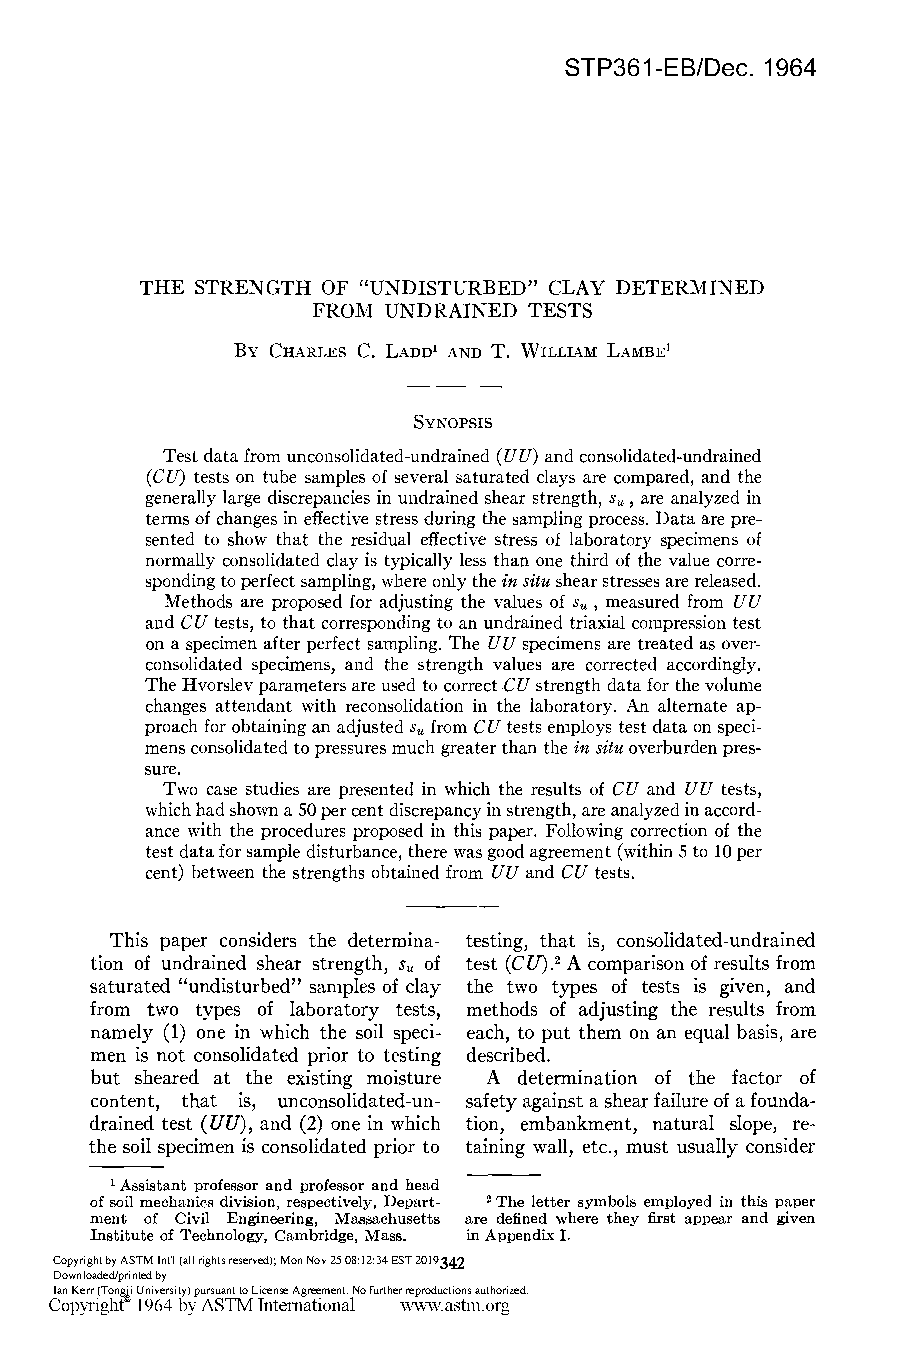
\includepdf[pages=1-30]{Ladd and Lambe 1966 -The strength of undisturbed clay determined from undrained test.pdf}

\end{document}